\documentclass{article}

\usepackage{amsmath, amsthm, amssymb, amsfonts}
\usepackage{thmtools}
\usepackage{graphicx}
\usepackage{setspace}
\usepackage{geometry}
\usepackage{float}
\usepackage{hyperref}
\usepackage[utf8]{inputenc}
\usepackage[english]{babel}
\usepackage{framed}
\usepackage[dvipsnames]{xcolor}
\usepackage{tcolorbox}

%Define the listing package
\usepackage{listings} %code highlighter
\usepackage{color} %use color
\definecolor{mygreen}{rgb}{0,0.6,0}
\definecolor{mygray}{rgb}{0.5,0.5,0.5}
\definecolor{mymauve}{rgb}{0.58,0,0.82}
 
%Customize a bit the look
\lstset{ %
backgroundcolor=\color{white}, % choose the background color; you must add \usepackage{color} or \usepackage{xcolor}
basicstyle=\footnotesize, % the size of the fonts that are used for the code
breakatwhitespace=false, % sets if automatic breaks should only happen at whitespace
breaklines=true, % sets automatic line breaking
captionpos=b, % sets the caption-position to bottom
commentstyle=\color{mygreen}, % comment style
deletekeywords={...}, % if you want to delete keywords from the given language
escapeinside={\%*}{*)}, % if you want to add LaTeX within your code
extendedchars=true, % lets you use non-ASCII characters; for 8-bits encodings only, does not work with UTF-8
frame=single, % adds a frame around the code
keepspaces=true, % keeps spaces in text, useful for keeping indentation of code (possibly needs columns=flexible)
keywordstyle=\color{blue}, % keyword style
% language=Octave, % the language of the code
morekeywords={*,...}, % if you want to add more keywords to the set
numbers=left, % where to put the line-numbers; possible values are (none, left, right)
numbersep=5pt, % how far the line-numbers are from the code
numberstyle=\tiny\color{mygray}, % the style that is used for the line-numbers
rulecolor=\color{black}, % if not set, the frame-color may be changed on line-breaks within not-black text (e.g. comments (green here))
showspaces=false, % show spaces everywhere adding particular underscores; it overrides 'showstringspaces'
showstringspaces=false, % underline spaces within strings only
showtabs=false, % show tabs within strings adding particular underscores
stepnumber=1, % the step between two line-numbers. If it's 1, each line will be numbered
stringstyle=\color{mymauve}, % string literal style
tabsize=2, % sets default tabsize to 2 spaces
title=\lstname % show the filename of files included with \lstinputlisting; also try caption instead of title
}
%END of listing package%
 
\definecolor{darkgray}{rgb}{.4,.4,.4}
\definecolor{purple}{rgb}{0.65, 0.12, 0.82}
 
%define Javascript language
\lstdefinelanguage{JavaScript}{
keywords={typeof, new, true, false, catch, function, return, null, catch, switch, var, if, in, while, do, else, case, break},
keywordstyle=\color{blue}\bfseries,
ndkeywords={class, export, boolean, throw, implements, import, this},
ndkeywordstyle=\color{darkgray}\bfseries,
identifierstyle=\color{black},
sensitive=false,
comment=[l]{//},
morecomment=[s]{/*}{*/},
commentstyle=\color{purple}\ttfamily,
stringstyle=\color{red}\ttfamily,
morestring=[b]',
morestring=[b]"
}
 
\lstset{
language=JavaScript,
extendedchars=true,
basicstyle=\footnotesize\ttfamily,
showstringspaces=false,
showspaces=false,
numbers=left,
numberstyle=\footnotesize,
numbersep=9pt,
tabsize=2,
breaklines=true,
showtabs=false,
captionpos=b
}

\colorlet{LightGray}{White!90!Periwinkle}
\colorlet{LightOrange}{Orange!15}
\colorlet{LightGreen}{Green!15}

\newcommand{\HRule}[1]{\rule{\linewidth}{#1}}

\NewEnviron{NORMAL}{% 
    \scalebox{2}{$\BODY$} 
} 

\declaretheoremstyle[name=Theorem,]{thmsty}
\declaretheorem[style=thmsty,numberwithin=section]{theorem}
\tcolorboxenvironment{theorem}{colback=LightGray}

\declaretheoremstyle[name=Proposition,]{prosty}
\declaretheorem[style=prosty,numberlike=theorem]{proposition}
\tcolorboxenvironment{proposition}{colback=LightOrange}

\declaretheoremstyle[name=Principle,]{prcpsty}
\declaretheorem[style=prcpsty,numberlike=theorem]{principle}
\tcolorboxenvironment{principle}{colback=LightGreen}

\setstretch{1.2}
\geometry{
    textheight=9in,
    textwidth=5.5in,
    top=1in,
    headheight=12pt,
    headsep=25pt,
    footskip=30pt
}

% ------------------------------------------------------------------------------

\begin{document}

% ------------------------------------------------------------------------------
% Cover Page and ToC
% ------------------------------------------------------------------------------

\title{ \normalsize \textsc{}
		\\ [2.0cm]
		\HRule{1.5pt} \\
		\LARGE \textbf{\uppercase{Programmazione e Algoritmica II SEMESTRE}
		\HRule{2.0pt} \\ [0.6cm] \LARGE{Corso C} \vspace*{10\baselineskip}}
		}
\date{}
\author{\textbf{Autore} \\ 
		Giuseppe Acocella \\
		2023/24\\}

\maketitle
\newpage

\tableofcontents

\newpage

\section{Strutture Dati}

Definiamo ed elenchiamo varie Strutture Dati che ci permettono di rappresentare degli insiemi dinamici.

\paragraph{Insieme Dinamico} Un Insieme Dinamico a differenza di Insiemi Statici hanno la caratteristica di poter essere modificati nel tempo. Rappresenteremo quindi ogni \textbf{elemento} dell'insieme come \textbf{oggetto} con dei relativi \textbf{attributi}. Perchè è necessario l'utilizzo di oggetti e attributi? Per poter sviluppare determinati insiemi dinamici sarà necessario \textbf{puntare} agli elementi successivi. In questo modo lavoreremo sempre per riferimento, puntando gli elementi tra di loro. Un esempio sono le linked list.

\paragraph{Operazioni su Insiemi Dinamici} Abbiamo due categorie di operazioni, ovvero le operazioni di \textbf{query} e le operazioni di \textbf{modifica}:

\begin{enumerate}
    \item Operazioni di Query: Le operazioni di Query "interrogano" la struttura dati, permettendo l'accesso ai suoi dati stessi. Sono delle operazioni di Query ad esempio SEARCH, MINIMUM, MAXIMUM, PREDECESSOR e SUCCESSOR.
    \item Operazioni di Modifica: Le operazioni di Modifica, appunto, modificano la struttura stessa e i dati al suo interno. Sono delle operazioni di modifica ad esempio INSERT e DELETE.
\end{enumerate}

\subsection{Strutture Dati Lineari}

Le strutture dati lineari sono caratterizzate da un "ordinamento" tra i vari suoi elementi, o meglio, sarà presente una relazione di successore e predecessore per ogni elemento.

\paragraph{Premessa sugli Array} Per poter permettere una prima implementazione di Pile e Code utilizzeremo degli Array. Ricordiamo alcune caratteristiche degli Array:
\begin{enumerate}
    \item Organizzazione Logica: L'organizzazione logica degli array è \textbf{contigua}. Dunque gli elementi sono in posizioni una successiva all'altra.
    \item Organizzazione Fisica: I valori sono memorizzati ad indirizzi \textbf{contigui}. In molti linguaggi infatti, per accedere ad un Array, si fa riferimento al primo elemento e successivamente si "somma al primo indice" la quantità necessaria per fare in modo che si possa accedere all'elemento desiderato.
    \item Costo delle operazioni: Possiamo quindi analizzare come il costo delle operazione su Array cambi in base a che tipo di operazione stiamo effettuando, se di \textbf{Query} o di \textbf{Modifica}. Infatti, facendo l'esempio nel quale volessimo rimuovere il terzo elemento da un array di 8 elementi (\textbf{Modifica}). Tutti gli elementi successivi a quello rimosso dovranno essere spostati, richiedendo quindi un costo \(O(n)\). Invece se volessimo accedere ad un elemento specifico (\textbf{Query}), basterebbe conoscere la sua posizione, richiedendo un costo $O(1)$.
\end{enumerate}

\newpage

\subsection{Stack (Pila)}

Gli stack sono strutture dati elementari caratterizzate dallo schema \textbf{LIFO}, ovvero Last In First Out. Potremmo implementare gli Stack su degli Array, ma andremmo ad incorrere naturalmente negli errori di \textbf{UNDER/OVER-FLOW}.

La pila infatti, se implementata su array, sarà gestita da un attributo \(S.top\) che indicherà l'elemento aggiunto più di recente. Le operazioni dunque di \textbf{Push} e \textbf{Pop} saranno gestite dallo spostamento di questo indice.

\begin{figure}[htbp]
    \center
    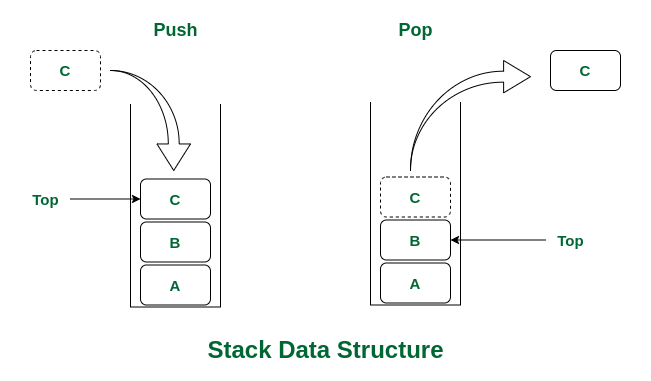
\includegraphics[scale=0.35]{img/stackImmagine.png}
\end{figure}

\begin{figure}[htbp]
    \center
    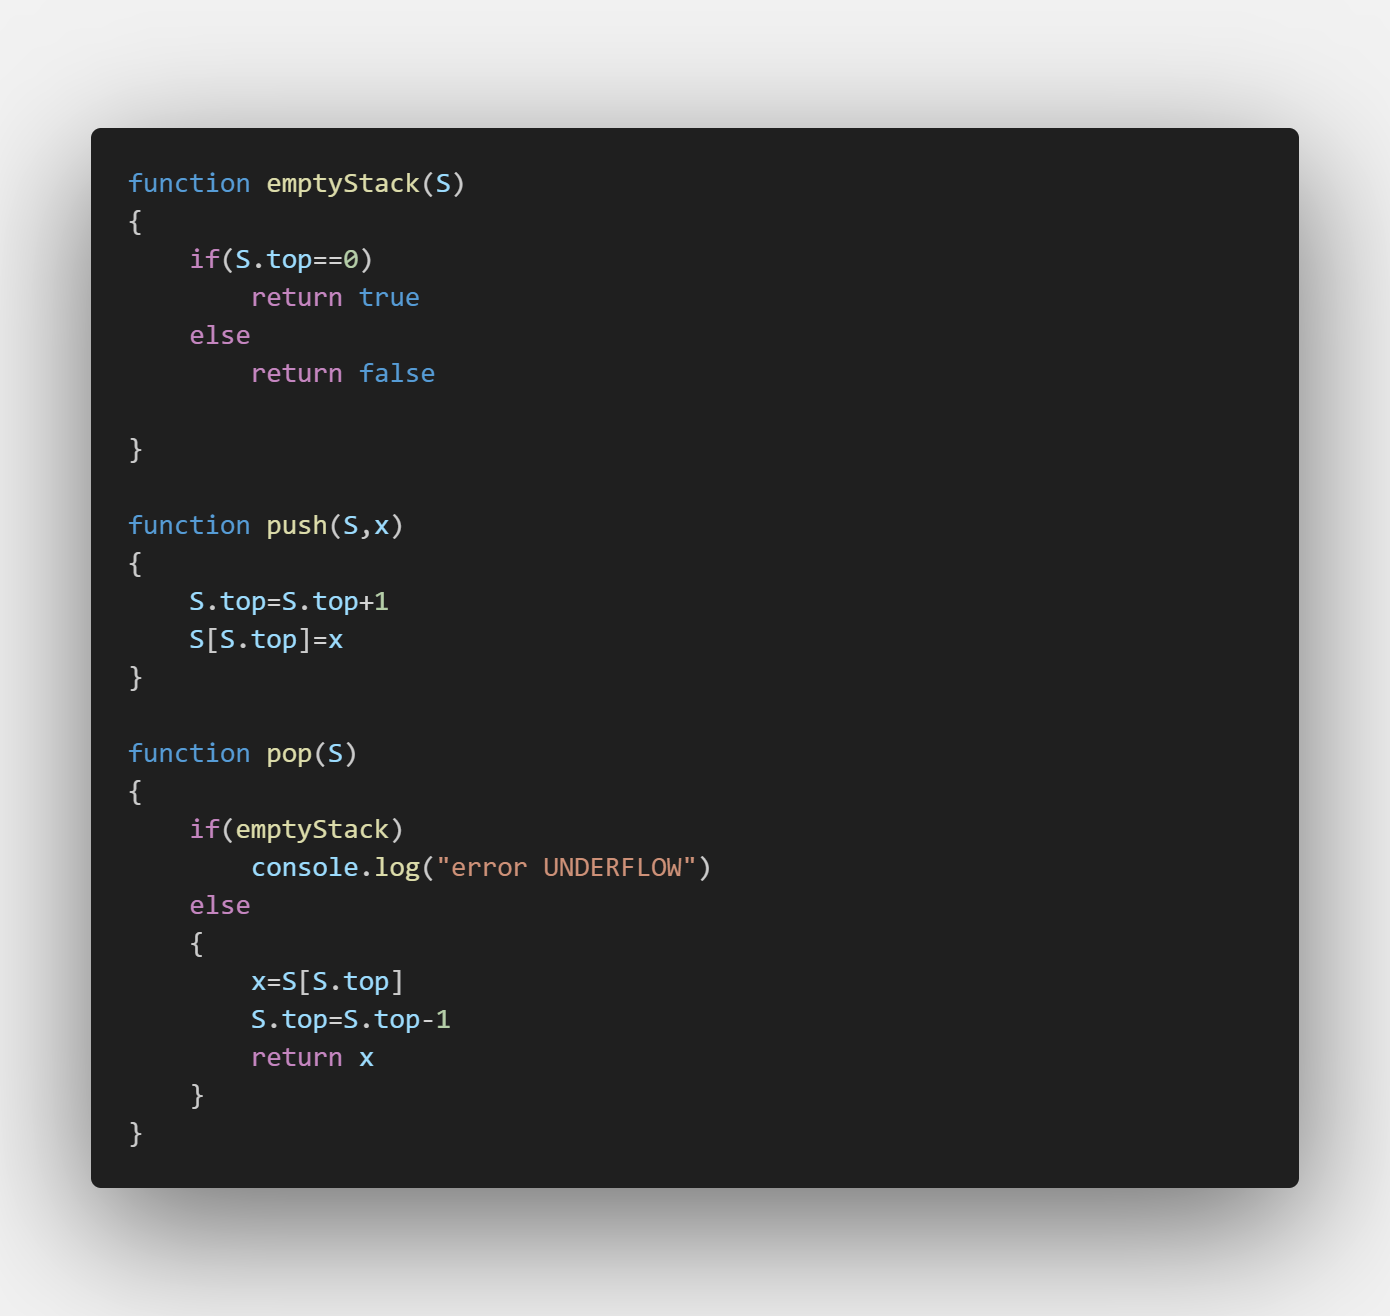
\includegraphics[scale=0.2]{img/stackOperazioni.png}
    \caption{Rappresentazione in pseudo-JS delle PILE su Array}
\end{figure}

\newpage

\subsection{Queue (Coda)}

Le Code sono strutture dati caratterizzate dallo schema \textbf{FIFO}, ovvero First In First Out. Possiamo implementare le Code su Array, e come per le Pile potremmo incorrere nella problematica di \textbf{UNDER/OVER-FLOW}. A differenza delle Pile, le Code utilizzano due attributi, ovvero \textbf{Q.head} e \textbf{Q.tail}, dove \(Q.head\) punta al primo elemento, ovvero quello da "più tempo" nella pila, mentre \(Q.tail\) punta la posizione successiva all'elemento aggiunto più di recente. 

\begin{figure}[htbp]
    \center
    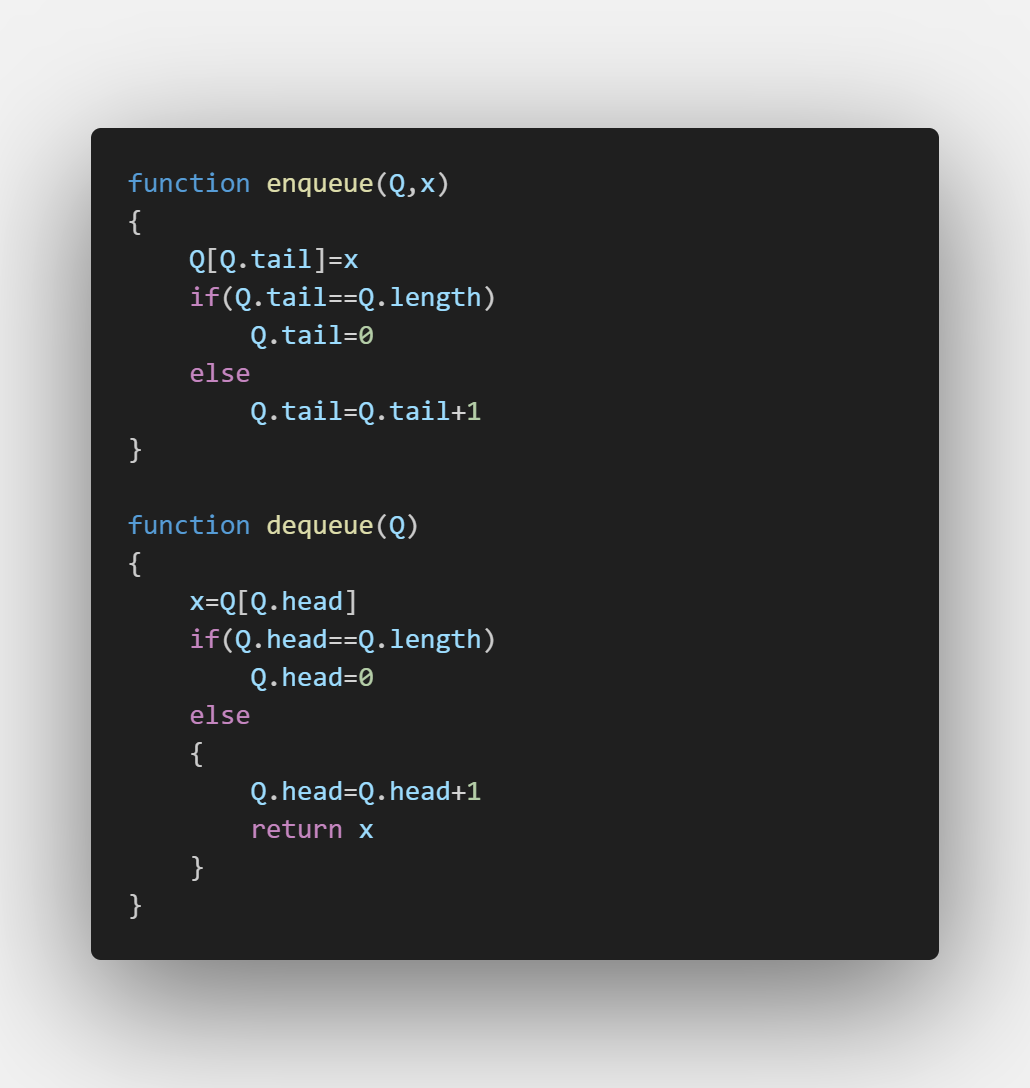
\includegraphics[scale=0.25]{img/queueOperazioni.png}
\end{figure}

\newpage

\subsection{Linked List Doppia}

Una linked list è una collezione di oggetti ognuno con tre attributi:
\begin{enumerate}
    \item Key: Attributo chiave, elemento effettivo quindi dell'oggetto in questione.
    \item Prev: Attributo puntatore, punta infatti all'elemento (oggetto) precedente.
    \item Next: Attributo puntatore, punta infatti all'elemento (oggetto) successivo.
\end{enumerate}

\begin{figure}[htbp]
    \center
    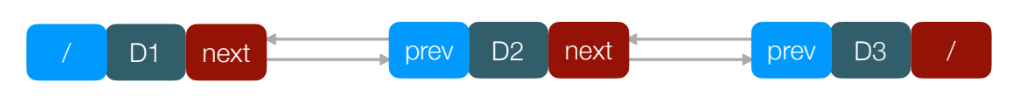
\includegraphics[scale=0.45]{img/linkedList.png}
\end{figure}

Ogni TRIPLA è dunque un oggetto con relativi attributi, definiamo quindi anche una LIST HEAD ed una LIST TAIL, determinate dall'assenza rispettivamente di un Prev o di un Succ.

\paragraph{Operazioni di Modifica e Costi} Notiamo che se vogliamo aggiungere un qualsiasi elemento in una qualsiasi posizione basterà cambiare i riferimenti di Prev e Next degli elementi tra cui vogliamo inserire il nuovo elemento. Questo provoca un costo \(O(1)\) in ogni tipologia di modifica, anche il \textbf{DELETE}.

\begin{figure}[htbp]
    \center
    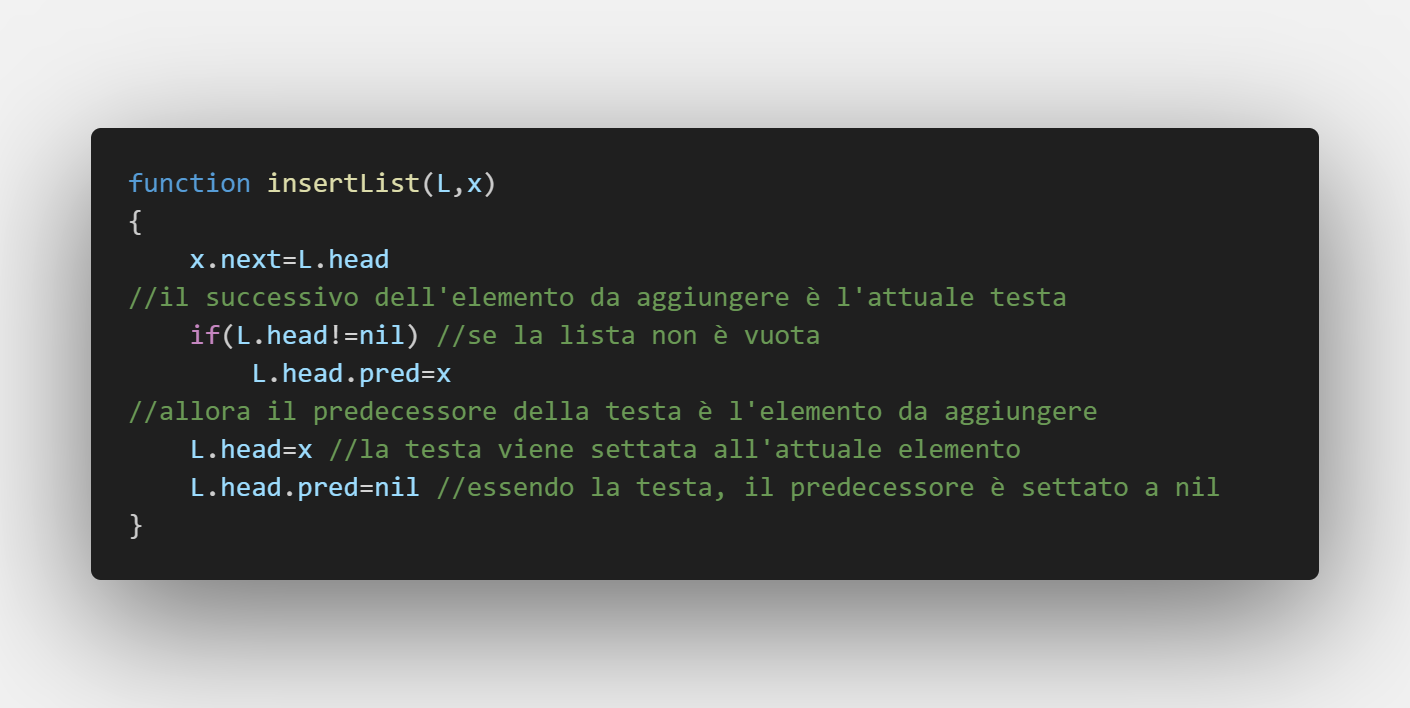
\includegraphics[scale=0.28]{img/queueOperazioni1.png}
\end{figure}

\newpage

\paragraph{Operazioni di Query e Costi} A differenza degli Array, queste strutture dati non sono logicamente contigue, dunque per accedere ad un elemento qualsiasi della lista sarà necessario "attraversare" tutti quelli ad esso precedenti.
Questo provocherà un costo O(n) per le operazioni di Query. 

\begin{figure}[htbp]
    \center
    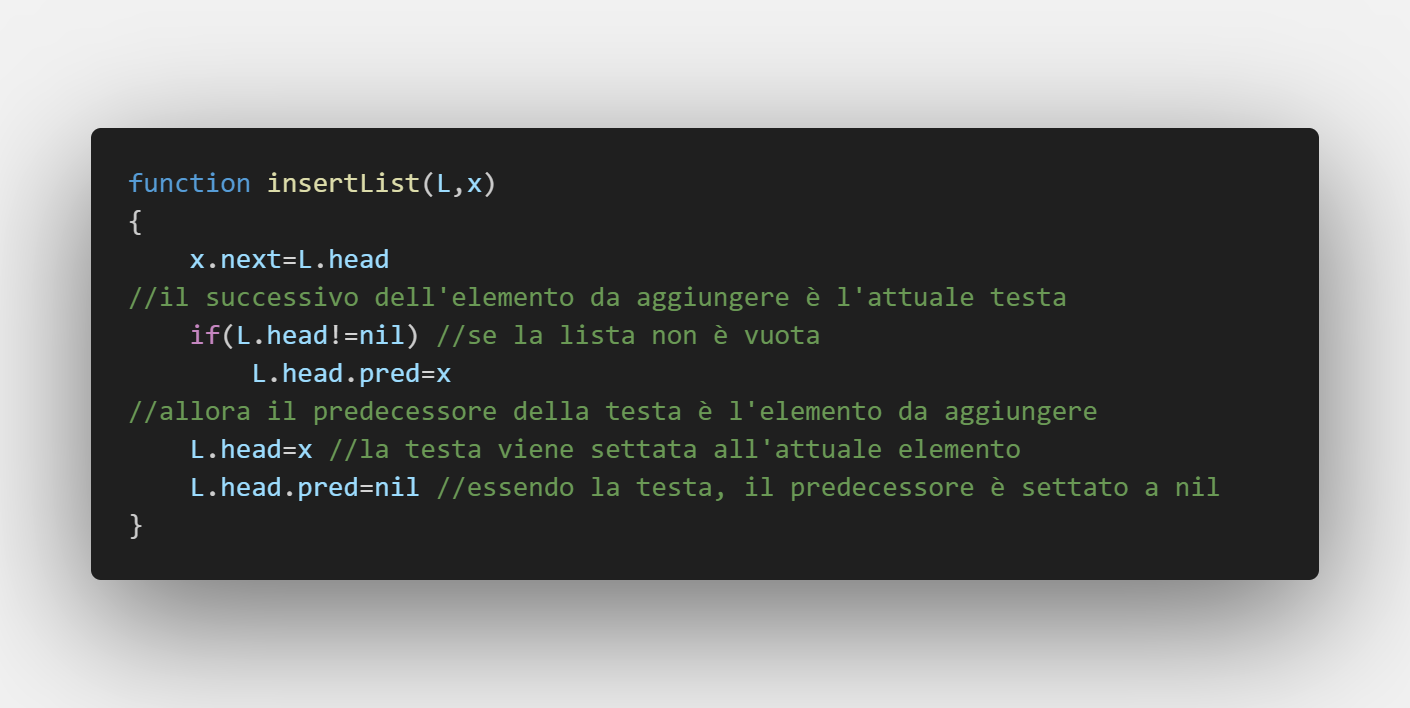
\includegraphics[scale=0.28]{img/queueOperazioni1.png}
\end{figure}

\paragraph{Rappresentazione di Elementi della Lista come Oggetti} Ecco una rappresentazione dove, ispirandoci alla sintassi di oggetto in JS, mostriamo ogni elemento come un oggetto con tre attributi, di cui 2 sono puntatori al precedente o al successivo. Attenzione, gli attributi puntatore non puntano agli attributi key dell'oggetto puntato, ma esattamente all'oggetto.

\begin{figure}[htbp]
    \center
    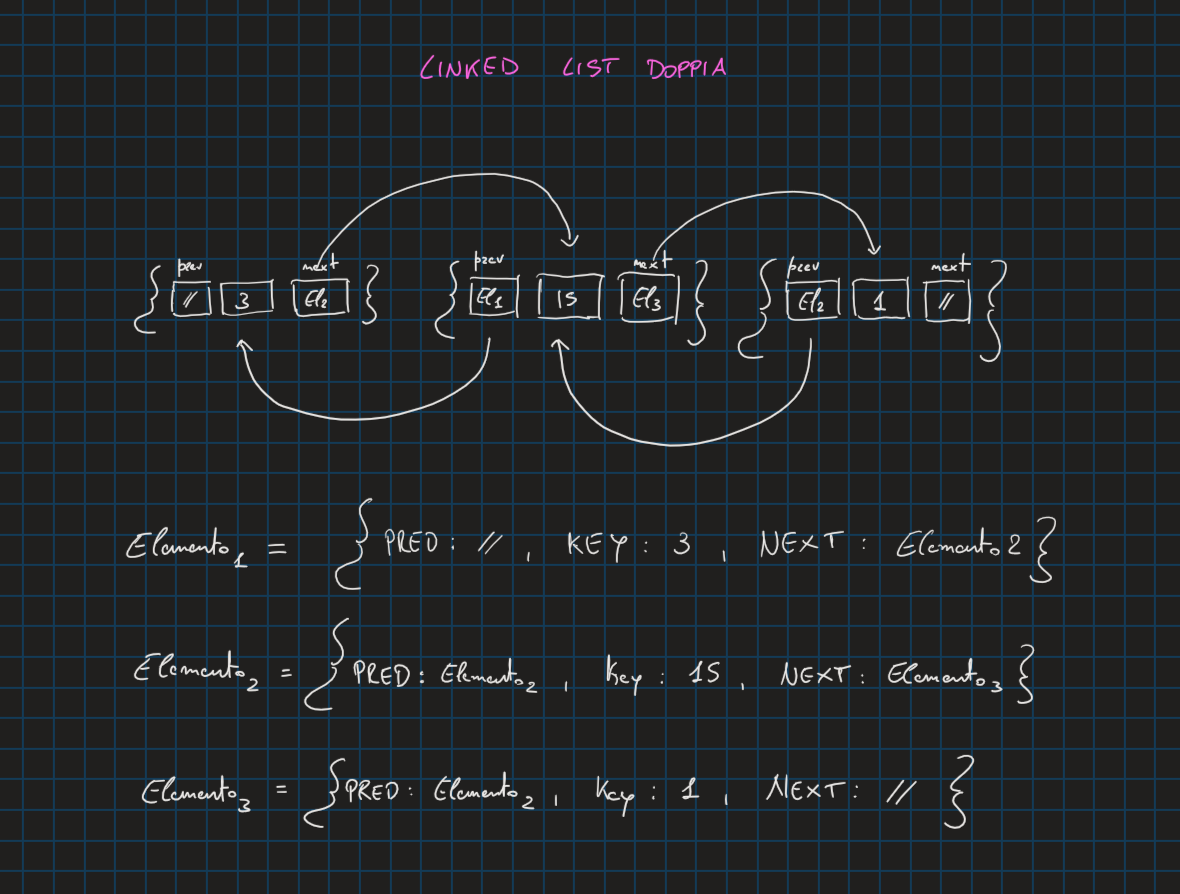
\includegraphics[scale=0.35]{img/imgLinkedList.png}
\end{figure}

\newpage

\paragraph{Gestione della Sentinella nelle Linked List} Per poter semplificare le operazioni agli estremi della lista, quindi le operazioni sui null, si potrebbe utilizzare un elemento nullo, ovvero la \textbf{sentinella}, impostata come precedente alla testa e successivo alla coda. Questo ci permette di evitare vari controlli durante le procedure di aggiunta e rimozione di elementi dalla lista.

\paragraph{Operazioni su liste con Sentinella} Mostriamo quindi le operazioni eseguite senza il controllo agli estremi delle liste. Ogni riferimento alla testa della lista verrà visto come successivo della sentinella quindi $L.nil.next$.

\begin{figure}[htbp]
    \center
    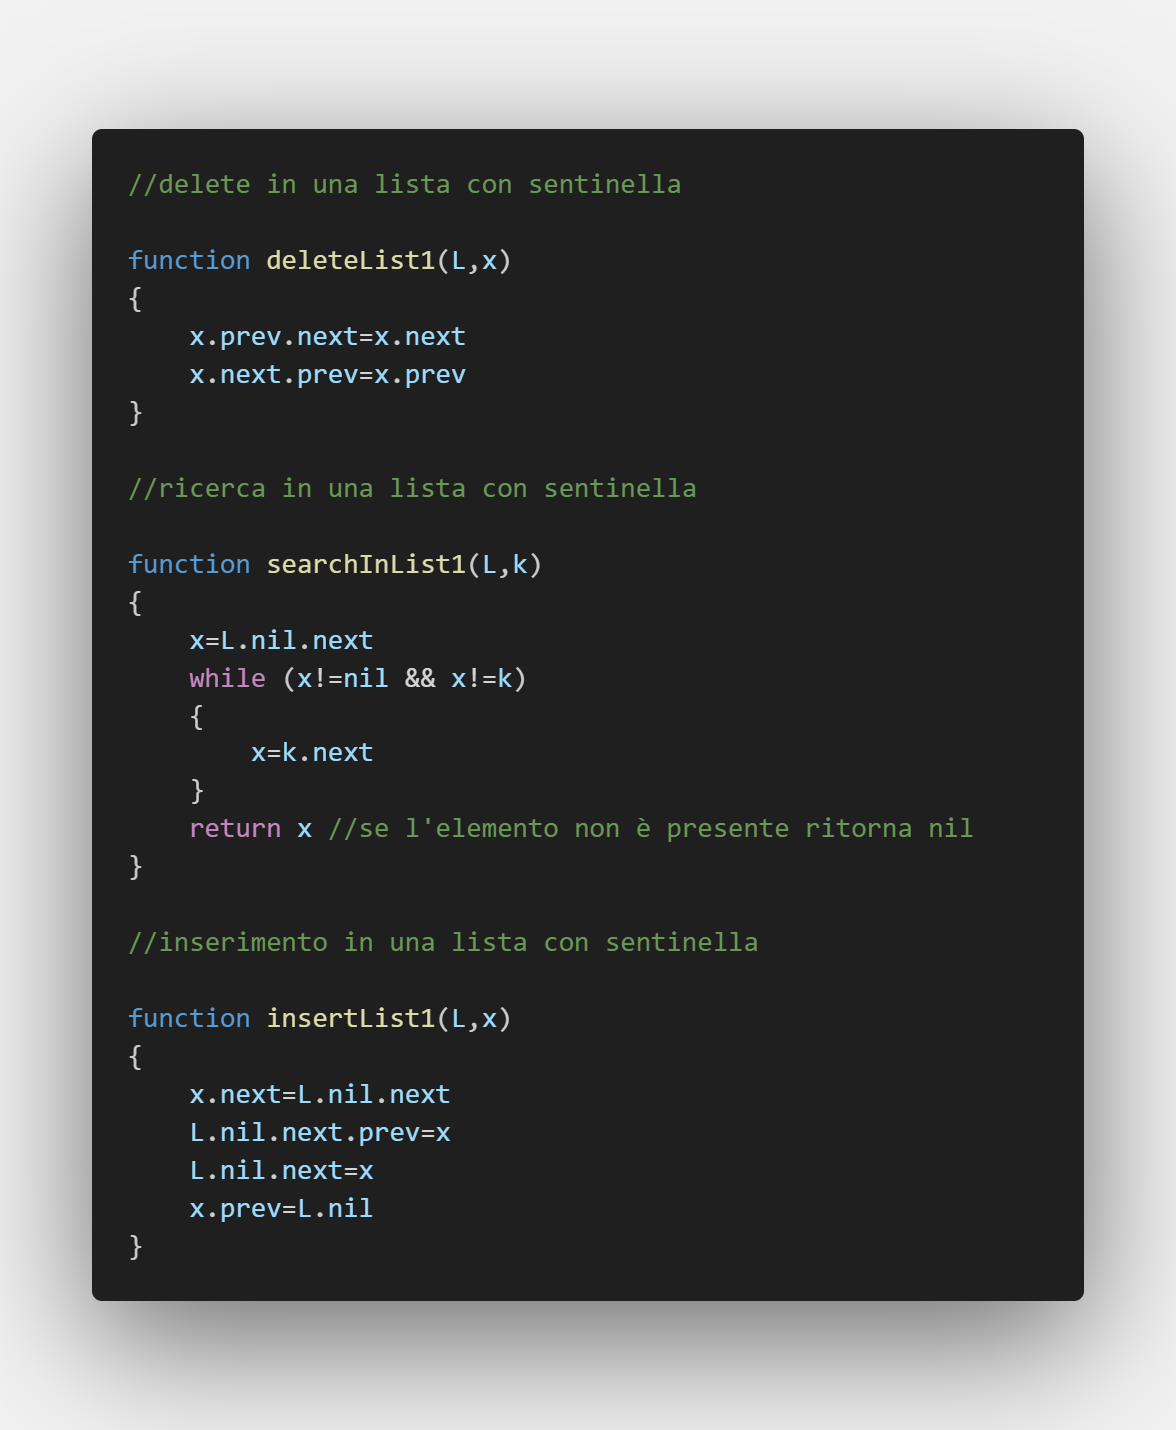
\includegraphics[scale=0.3]{img/operazioniSentinella.png}
\end{figure}

\newpage

\subsubsection{Esempi d'applicazione} Mostriamo degli esempi di esercizi che utilizzano strutture dati lineari per ottimizzare le operazioni:

\paragraph{Notazione Polacca Inversa} La notazione polacca inversa è una forma che permette di annullare ogni tipo di ambiguità ponendo gli operandi prima dell'operatore. Potremmo immaginarci gli operandi come "argomenti" posti prima dell'operazione che li elaborerà. Mostriamo un esempio.

\begin{equation}
\NORMAL{(((2+3)*7)-5)}
\end{equation}

\begin{figure}[htbp]
    \center
    
\includegraphics[scale=0.5]{img/NPI.png}
\end{figure}

Come possiamo implementare un algoritmo che legga questa notazione e che la valuti?

Descriviamo passo passo le operazioni da eseguire:

\begin{enumerate}
    \item Leggo da sinistra verso destra l'espressione ed eseguo un $push()$ nella pila quando trovo degli operandi
    \item Quando trovo un operatore eseguo due $pop()$ nella pila, valutando quell'operazione
    \item Una volta eseguita l'operazione, eseguo un $push()$ alla pila con il risultato ottenuto
    \item Reitero fino a quando non rimane un solo elemento nella pila, ovvero il risultato. Ovviamente stiamo considerando di aver valutato l'intera espressione.
\end{enumerate}

Mostriamo dunque un'implementazione in JavaScript del seguente algoritmo, assumendo l'utilizzo della seguente classe:

\begin{lstlisting}[language=JavaScript]
    constructor(){
        this.top=0
        this.data=[]
    }
    isEmpty(){
        return this.top===0?true:false
\end{lstlisting}

\begin{lstlisting}[language=JavaScript]
    push(element){
        this.top++
        this.data[this.top]=element
    }
    pop(){
        if(!this.top<=1)
        {
            this.top=this.top-1
            return this.data[this.top+1]
        }
        else
            return "UNDERFLOW ERROR"
    }
\end{lstlisting}

\newpage

\begin{lstlisting}[language=JavaScript]
function npi (espressione)
{
    let pila1 = new Stack();
    let opr1,opr2,res
    for(let i of espressione)
    {
        switch(i)
        {
            case "+":
                opr2=pila1.pop()
                opr1=pila1.pop()
                res= Number(opr1)+Number(opr2)
                pila1.push(""+res)
                break;

            case "-":
                opr2=pila1.pop()
                opr1=pila1.pop()
                res= Number(opr1)-Number(opr2)
                pila1.push(""+res)
                break;

            case "*":
                opr2=pila1.pop()
                opr1=pila1.pop()
                res= Number(opr1)*Number(opr2)
                pila1.push(""+res)
                break;

            case "/":
                opr2=pila1.pop()
                opr1=pila1.pop()
                res= Number(opr1)/Number(opr2)
                pila1.push(""+res)
                break;

            default:
                pila1.push(i)
        }
    }
    return pila1.data[1]
} 
\end{lstlisting}

%\begin{figure}[htbp]
%    \center
%   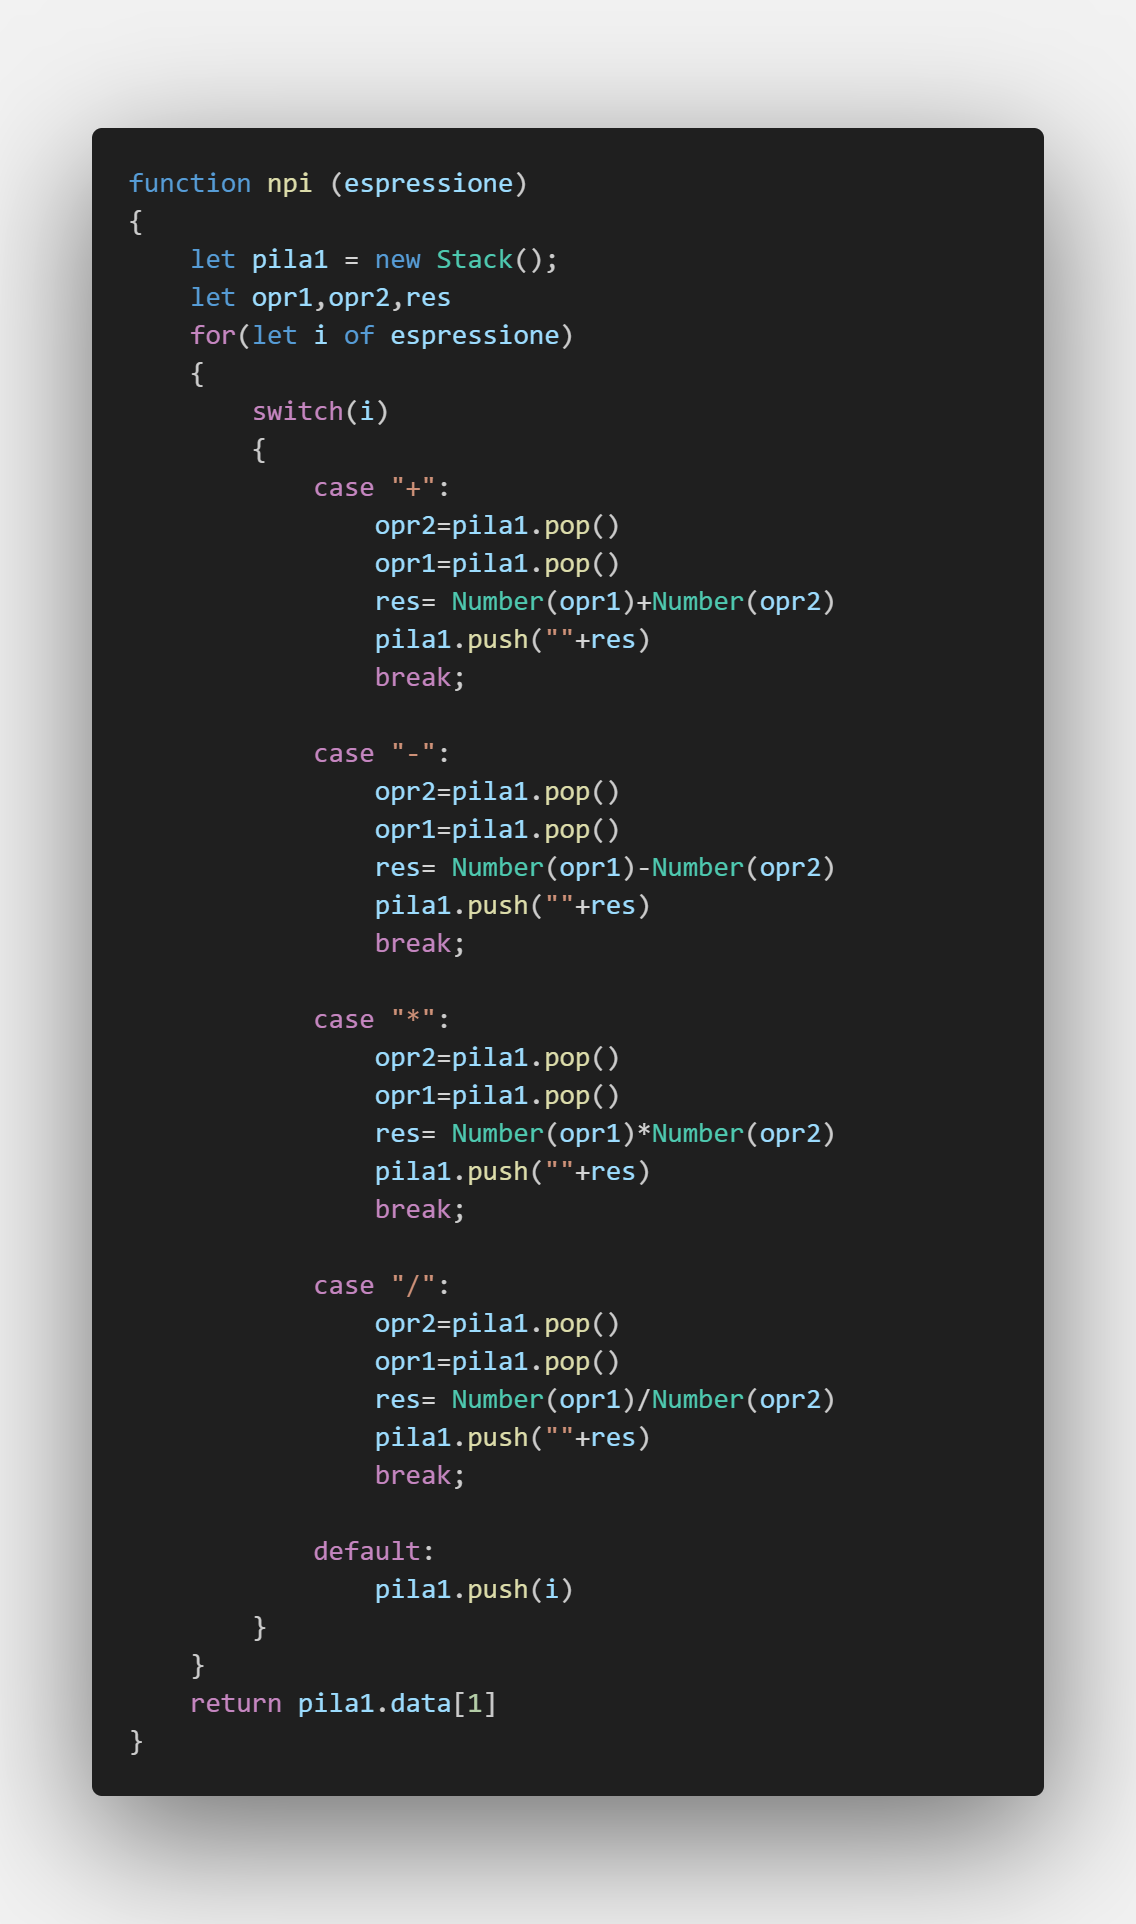
\includegraphics[scale=0.32]{img/jsNPI.png}
%\end{figure}

\newpage

\paragraph{Visita Livelli albero con coda} Possiamo mostrare un altro esempio di utilizzo di strutture dati lineari. Infatti la visita per livelli di un albero k-ario in questo caso viene implementata grazie ai seguenti passi:

\begin{enumerate}
    \item Valuta la radice, carica quindi nella coda i suoi figli ed effettua un $dequeue()$ sulla testa che contiene l'attuale radice per poter proseguire, accumuliamo quindi le varie teste delle code che vengono rimosse
    \item Reiteriamo questa operazione su tutti gli elementi della coda fino al raggiungimento della coda vuota
\end{enumerate}

Dunque in questo caso abbiamo utilizzato questa classe per l'implementazione delle code:

\begin{lstlisting}[language=JavaScript]
    class Queue
{
    constructor()
    {
        this.head=0
        this.tail=0
        this.data=[]
    }

    isEmpty(){
        if(this.tail==this.head)
            return true
        else
            return false
    }


    enqueue(element){
        this.data[this.tail]=element
        this.tail=this.tail+1
    }

    dequeue(){
        this.head=this.head+1
        return this.data[this.head-1]
    }
}
\end{lstlisting}

Mostriamo quindi l'algoritmo in JavaScript. (La corrente implementazione non è ottimale, infatti è in ordine \(O(n^2)\).

\newpage

\begin{lstlisting}[language=JavaScript]

function visitaLivelli(tree)
{
    let res=[]
    let coda1 = new Queue();
    coda1.enqueue(tree)

    while (!coda1.isEmpty())
    {
        let elementoElab = coda1.dequeue()
        res.push(elementoElab.val)
        if(elementoElab.s)
        {
            for(let j in elementoElab.s)
                coda1.enqueue(elementoElab.s[j])
        }
    }

    return res
}

\end{lstlisting}

\subsection{Strutture Dati Non Lineari}

Fino ad ora abbiamo descritto strutture come Array, Liste, Pile e Code, dove ha senso chiederci quale sia l'elemento successivo e quello precedente. In questo capitolo descriveremo invece strutture come Alberi o Tavole Hash che non sono lineari.

\subsection{Alberi - Definizione} Possiamo definire gli alberi come una struttura dati gerarchica, caratterizzata appunto tra "relazioni" tra nodi. Elenchiamo alcuni tratti caratteristici di questa struttura dati:

\begin{enumerate}
    \item Radice: Nodo senza padre.
    \item Nodi Fratelli: Nodi che hanno lo stesso padre.
    \item Profondita di Nodo: Numero di antenati del nodo stesso.
    \item Altezza dell'albero: Profondità massima di un nodo nell'albero.
\end{enumerate}

\begin{figure}[htbp]
    \center
    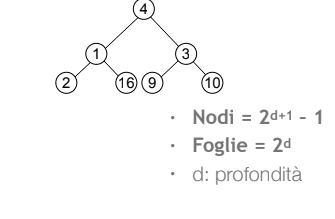
\includegraphics[scale=0.75]{img/alberoBinCompleto.png}
\end{figure}

\newpage

\paragraph{Visite Alberi e Possibili Implementazioni}

Una volta denotata la struttura "logica" di un albero, ci chiediamo come questi si possano implementare effettivamente. Mostriamo degli esempi:

\begin{enumerate}
    \item Alberi implementati su Array: Questa implementazione è la più semplice, e porta diversi svantaggi.

    \begin{figure}[htbp]
        \center
        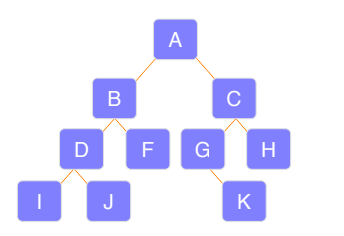
\includegraphics[scale=0.75]{img/alberoBinarioArray1.png}
        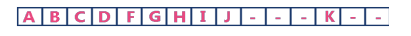
\includegraphics[scale=0.75]{img/alberoBinarioArray2.png}
    \end{figure}

    Infatti, anche se le operazioni di accesso sono dirette, il $search()$ sarebbe in ordine $O(n)$
    e saremmo costretti ad investire spazio inutilmente per le celle che devono indicare i "\(nil"\) dei nodi senza figli.

    \item Alberi implementati su Linked List

    \begin{figure}[htbp]
        \center
        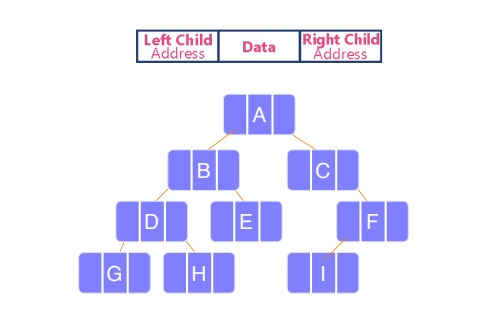
\includegraphics[scale=0.75]{img/listaAlbero.png}
    \end{figure}

    Questo tipo di implementazione non spreca spazio, e ci permette anche di modificare abbastanza facilmente l'albero grazie all'utilizzo dei riferimenti. (Questa implementazione è molto simile a quella che si utilizza solitamente per gli alberi binari in JavaScript).
    
\end{enumerate}

\newpage

\paragraph{Tipologie di Visite di Alberi Binari} Descriviamo prima di tutto le possibili visite che si possono effettuare su un albero binario tenendo in considerazione il nodo, il figlio sx e il figlio dx.

\begin{enumerate}
    \item Visita Anticipata (PreOrder): NODO - FIGLIO SX - FIGLIO DX
    \item Visita Simmetrica (InOrder): FIGLIO SX - NODO - FIGLIO DX
    \item Visita Asimmetrica (PostOrder): FIGLIO SX - FIGLIO DX - NODO
\end{enumerate}

\subsection{Alberi Binari di Ricerca}

Gli Alberi Binari di Ricerca (ABR) sono caratterizzati dall'ordine dei dati al suo interno. Per essere definito come tale, infatti, un albero binario di ricerca deve rispettare queste 2 condizioni:

\begin{enumerate}
    \item Esiste una relazione di ordinamento totale tra i valori al suo interno, dunque è sempre possibile stabilire chi precede l'altro e viceversa.
    \item Per ogni nodo e relativo valore, alla sua sinistra appariranno solo valori inferiori, e a destra solo valori superiori.
\end{enumerate}

\begin{figure}[htbp]
        \center
        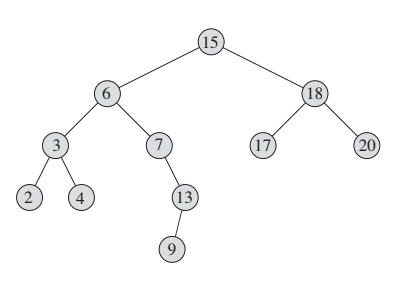
\includegraphics[scale=0.75]{img/ABR.png}
    \end{figure}

\subsubsection{Operazioni su ABR} Le operazioni di Query e di Modifica notiamo che sono caratterizzate dal bilanciamento dell'albero stesso. Mostriamo qualche esempio.

\paragraph{Ricerca su ABR} La ricerca si baserà sull'ordinamento dell'albero stesso. Dunque, partendo dalla radice, se il valore cercato è più grande di quello attuale, allora si cercherà nel sottoalbero destro, altrimenti in quello sinistro. Reiterando questo procedimento ritroveremo il numero cercato, se presente. Costo dell'operazione? $O(h)$.

\newpage

\paragraph{Max/Min su ABR} In base a se stiamo cercando massimo o minimo, andremo a cercare arbitrariamente e rispettivamente a destra o a sinistra. Costo? $O(h)$.

\paragraph{Inserimento in ABR} Un nuovo nodo verrà sempre inserito come foglia, ma il suo inserimento dovrà sempre rispettare la seconda condizione che caratterizza gli ABR. Costo? $O(h)$.

\begin{figure}[htbp]
        \center
        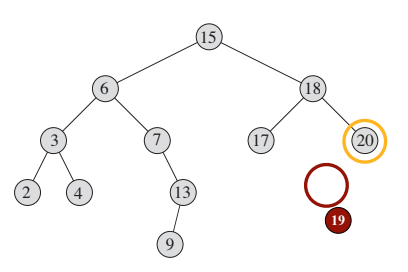
\includegraphics[scale=0.75]{img/inserimentoABR.png}
    \end{figure}

\paragraph{Altezza, Bilanciamento ed Efficienza} Notiamo che tutte le operazioni mostrate precedentemente, dipendevano fortemente dall'altezza dell'albero stesso. Non possiamo però affermare che l'altezza rispetterà sempre un ordine logaritmico. Se ponessimo il caso in cui i dati inseriti siano già stati ordinati, allora staremmo sviluppando un albero completamente sbilanciato, tendendo quasi ad una lista.

\begin{figure}[htbp]
        \center
        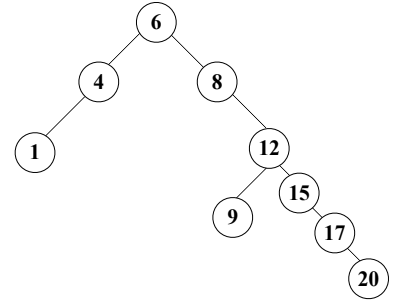
\includegraphics[scale=0.6]{img/bilanciamentoABR.png}
    \end{figure}

Notiamo quindi che per preservare i vantaggi stabiliti da un albero binario di ricerca, è necessario mantenere una condizione semi-bilanciata, che assomigli il più possibile ad un albero binario completo. Esistono dei metodi di bilanciamento diretti, che redistribuiscono i valori periodicamente per assicurarne la corretta distribuzione, ma questo problema viene risolto completamente nei 2-3 Alberi.

\newpage

\subsection{2-3 Alberi} Questa struttura dati risolve la questione del bilanciamento degli ABR grazie ad una sorta di compromesso. Esprimiamo le condizioni che caratterizzano questa struttura:

\begin{enumerate}
    \item Tutti i nodi hanno almeno 2 figli e massimo 3.
    \item Tutti i cammini radice-foglia hanno la stessa lunghezza.
\end{enumerate}

\subsubsection{Lemma su n(nodi), f(foglie) e h(altezza)} definiamo questo lemma con queste due condizioni:

\begin{enumerate}
\item Prima condizione:
\begin{equation}
    2^{h+1}-1 \leq n \leq \frac{(3^{h+1}-1)}{2}
\end{equation}

\item Seconda condizione:
\begin{equation}
    2^h \leq f \leq 3^h
\end{equation}

\end{enumerate}

Questo quindi ci permette di sviluppare una dimostrazione per induzione che ci permette di affermare che in ogni caso il costo sarà $\Theta(log n)$.

\paragraph{Dimostrazione per Induzione} Definiamo passo passo la dimostrazione:

\begin{enumerate}
    \item Caso Base: Considerando un albero di altezza $h=0$ staremmo semplicemente ipotizzando un caso banale che ci permette di assicurare che la proprietà sia vera per h=0
    \item Caso induttivo: Assumiamo che $P(n)$ sia vera e verifichiamo che sia vera 
    
    anche $P(n+1)$. Sappiamo che se validiamo quest'implicazione, allora sarà valida per ogni $n$.
    Per poter validare l'implicazione, consideriamo un $T$ albero con altezza $h+1$, allora:

    \begin{enumerate}
        \item Sia $T^{'}$ un albero ottenuto sottraendo a $T$ l'ultimo livello
        \item Siano $f^{'}$ e $n^{'}$ rispettivamente foglie e nodi di $T^{'}$
        \item Per ipotesi induttiva avremo $2^{h+1}-1 \leq n^{'} \leq \frac{(3^{h+1}-1)}{2}$ e $2^h \leq f^{'} \leq 3^h$
        \item Allora dato che ogni foglia in $T^{'}$ avrà tra due e tre figli in $T$ avremo
        
        che $2*2^h \leq f \leq 3*3^h$ ovvero $2^{h+1} \leq f \leq 3^{h+1}$
        \item Dato che $n=n+f^{'}$ abbiamo completato la dimostrazione
    \end{enumerate}
    
\end{enumerate}

\begin{figure}[htbp]
        \center
        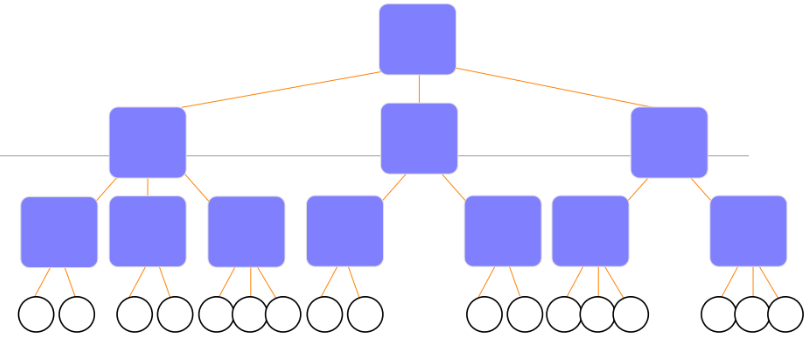
\includegraphics[scale=0.4]{img/2-3Alberi.png}
\end{figure}

\newpage

\paragraph{Ordine e Distribuzione Dati nei 2-3 Alberi} Durante l'inserimento dei dati, la struttura del 2-3 Albero "indirizza" il valore in base all'intervallo a cui deve appartenere. Infatti i dati dell'albero verranno distribuiti in "intervalli" spezzati dai valori \(S[v]\) e \(M[v]\).

\begin{enumerate}
    \item $S[v]$ indica l'elemento maggiore del sottoalbero sinistro
    \item $M[v]$ indica l'elemento minore del sottoalbero destro
\end{enumerate}

Utilizzeremo questi due elementi per "spezzare" i dati ordinati all'interno dell'albero per suddividere in "intervalli" i dati stessi.

\begin{figure}[htbp]
        \center
        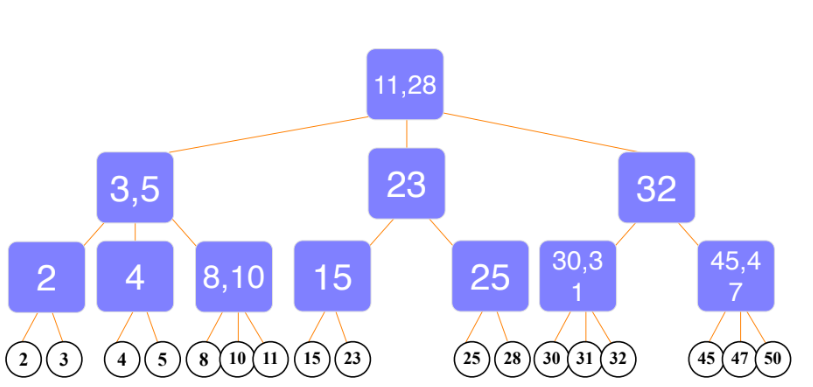
\includegraphics[scale=0.45]{img/alberi2-3.png}
\end{figure}

\begin{figure}[htbp]
        \center
        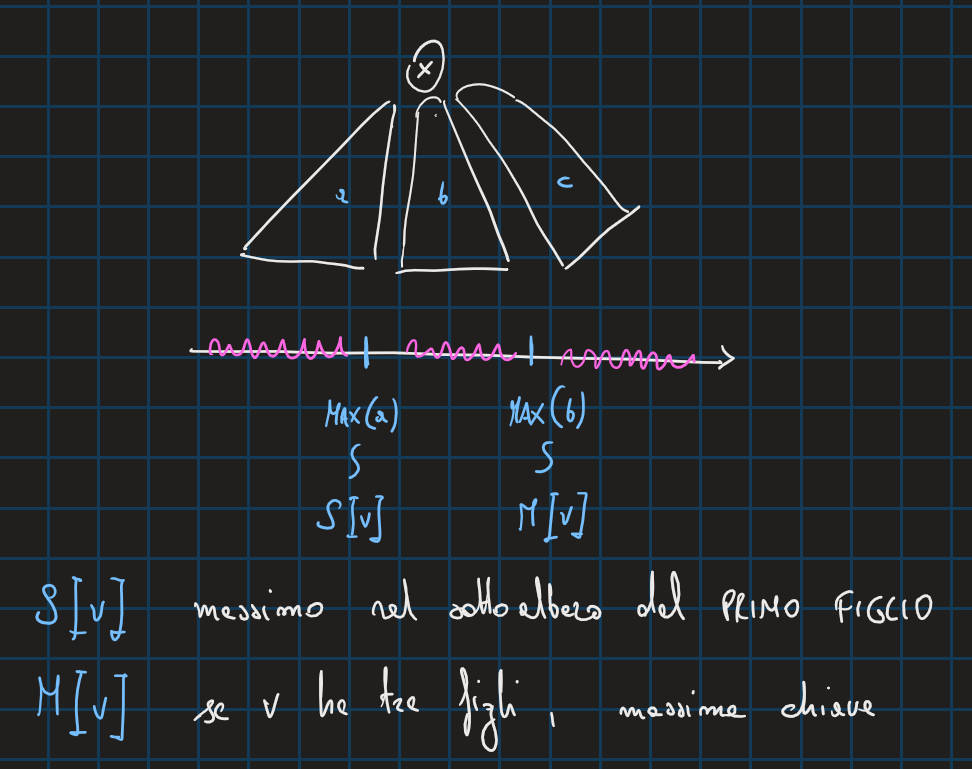
\includegraphics[scale=0.45]{img/distribuzione2-3.png}
\end{figure}

Questa distribuzione ci permette di avere una struttura sempre bilanciata. Il vantaggio del bilanciamento della struttura è che $h=\Theta(log n)$. Ricordiamo infatti che tutte le operazioni definite su questa struttura e sull'ABR dipendono fortemente dall'altezza. Dunque è nostro interesse "forzare" l'altezza ad ordine logaritmico.

\newpage

\subsubsection{Operazioni su 2-3 Alberi} Dato che questo tipo di struttura permette di ottimizzare tutti i costi delle operazioni di query/modifica, si presenta la necessità di descrivere bene il mantenimento di questa struttura e le sue proprietà.

\paragraph{Search su 2-3 Alberi} Descriviamo lo pseudocodice sottostante:

Notiamo subito che il tipo di ricerca che stiamo effettuando è ricorsiva.
In un albero 2-3, ogni gruppo di dati ordinati, può essere suddiviso in 2 o 3 intervalli.
Allora effettuiamo questi controlli

\begin{enumerate}
    \item Controllo che la radice non sia una foglia, quindi sto controllando il caso base della ricorsione
    \begin{enumerate}
        \item Controllo che il valore cercato non sia nella radice
    \end{enumerate}
    \item Stabilisco, utilizzando gli elementi $S[v]$ e $M[v]$, quale sia l'intervallo da controllare:
    \begin{enumerate}
        \item Quello sinistro o destro se la radice ha due figli
        \item Il primo, il secondo o il terzo se la radice ha tre figli
    \end{enumerate}
\end{enumerate}

\newpage

\begin{lstlisting}[language=JavaScript]

function search(radice,valore)
{
	if(radice == una foglia)
	{
		if(valore == chiave(radice))
			return chiave(radice)
		else
			return null
	}
	else
	{
		v_i=figlio(radice)
		if(valore < S[radice])
		{
			search(v1,valore)
		}
		else
		{
			if(radice ha due figli || valore < M[radice])
			{
				search(v2,valore)
			}
			else
			{
				search(v3,valore)
			}
		}
	}
}

\end{lstlisting}

\newpage

\paragraph{Insert/Delete e Split} Ipotizziamo di dover aggiungere un nuovo valore all'albero 2-3 tra le foglie. Abbiamo 2 possibili casi:

\begin{enumerate}
    \item Trovato il potenziale nodo padre, questo ha 2 figli, quindi possiamo aggiungerlo senza particolari problemi
    \item Trovato il potenziale nodo padre, questo ha 3 figli, dunque aggiungendo una foglia andremmo a violare la proprietà 2-3. Risulta quindi necessaria una procedura che ristabilizzi la condizione 2-3 dopo aver creato un nodo padre con 4 figli
\end{enumerate}

\paragraph{Descrizione della procedura di Split}

Descriviamo dunque lo split, considerando 3 elementi principali, ovvero:
\begin{enumerate}
    \item Nodo $v$ padre
    \item Nodo $w$ nuovo
    \item Nodo $u$ aggiunta
\end{enumerate}

Una volta identificati questi elementi principali, possiamo descrivere a passi l'algoritmo, sapendo che l'obiettivo è quello di collocare correttamente il nodo $u$ aggiunta.

\begin{enumerate}
    \item Identificate le foglie del nodo $v$ padre, le sue due foglie con chiave minima diventano figlie di nodo $w$ nuovo
    \item Le due rimanenti foglie di nodo $v$ padre restano a v
    \item Il nodo $w$ nuovo viene attaccato al padre del nodo $v$ padre
    \item Se il padre di nodo $v$ padre adesso ha 3 figli va bene, altrimenti dobbiamo richiamare la funzione split anche su padre di $v$
\end{enumerate}
\begin{figure}[htbp]
        \center
        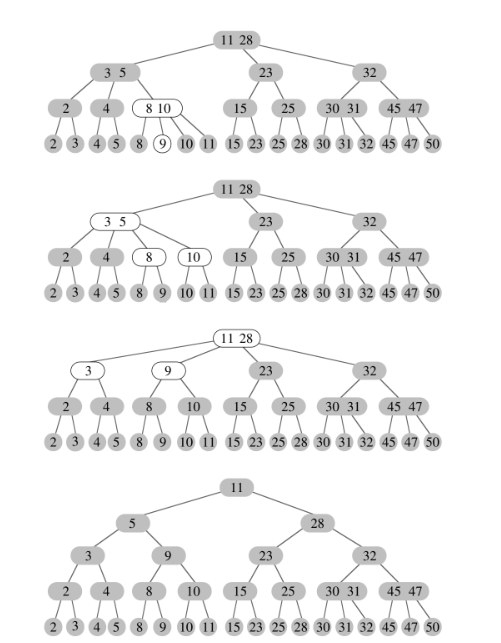
\includegraphics[scale=0.5]{img/imgSplit23.png}
\end{figure}
\newpage

\subsection{Heap}

Un heap è caratterizzato dalla presenza di due proprietà fondamentali:

\begin{enumerate}
    \item \textbf{Proprietà Strutturale di Albero Quasi Completo,} ovvero un albero completo, tranne l'ultimo livello dove le foglie si distribuiscono in maniera non bilanciata tra sinistra e destra

    \begin{figure}[htbp]
        \center
        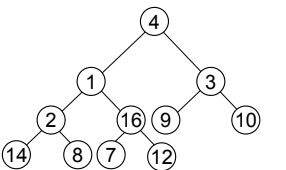
\includegraphics[scale=0.7]{img/alberoQuasiCompleto.png}
    \end{figure}

    \item \textbf{Proprietà di Max/Min Heap}, ovvero la radice di ogni sottoalbero è il massimo o il minimo tra i nodi del sottoalbero stesso. E' detto maxHeap quando la radice è il massimo del sottoalbero e minHeap quando la radice è il minimo del sottoalbero.

\end{enumerate}

\subsubsection{Implementazione su Array} Dato che l'albero non avrà "buchi", l'implementazione naturale dell'heap è su array, dato che la parte vuota sarà quella sulla destra. Distribuiamo quindi i valori dei nodi per livelli nell'array.

\begin{figure}[htbp]
        \center
        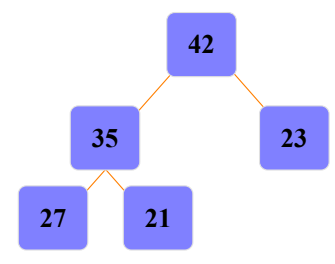
\includegraphics[scale=0.5]{img/heap1.png}
    \end{figure}

\begin{figure}[htbp]
        \center
        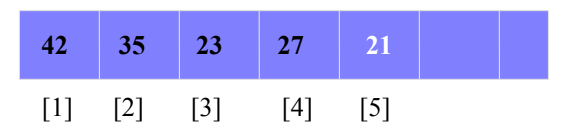
\includegraphics[scale=0.5]{img/heap2.png}
        \caption{Implementazione su array con indici da 1}
    \end{figure}

\paragraph{Indici Padre/Figlio} Notiamo che esprimendo in questi termini l'heap, è possibile determinare in questo modo le relazioni esistenti tra i nodi:

\begin{enumerate}
    \item $indicePadre = floor(indiceElemento/2)$
    \item $indiceFiglioSx = 2*indicePadre$
    \item $indiceFiglioDx = (2*indicePadre)+1$
\end{enumerate}

\newpage

\subsubsection{Operazioni su Heap} Definiamo varie operazioni su questa struttura dati, come quella per mantenere la condizione di maxHeap o quella per costruire un maxHeap a costo lineare, ma prima è necessario ricordare queste due concetti fondamentali:

\begin{enumerate}
    \item L'\textbf{altezza} di un nodo si considera dal basso verso l'alto
    \item La \textbf{profondità} di un nodo si considera dall'alto verso il basso
\end{enumerate}

\subsubsection{maxHeapify} Aggiungendo un nodo o modificando in qualche modo i dati all'interno dell'heap potremmo alterarne la condizione di maxHeap. Dobbiamo costantemente controllare quindi che questa condizione sia rispettata affinchè si possano sfruttare tutti i vantaggi generati dall'Heap.

Descriviamo dunque a passi l'algoritmo di maxHeapify:

\begin{enumerate}
    \item Si assume che i sottoalberi sx e dx correnti rispettino la condizione di maxHeap
    \item Si controlla dunque se l'attuale radice rompe la condizione
    \item In caso affermativo, si esegue uno swap con il maggiore tra i figli sx e dx
    \item Si ricontrolla, sull'albero la cui radice è stata swappata che sia rispettata la condizione di maxHeap
    \item In caso negativo si richiama ricorsivamente la funzione maxHeapify sul sottoalbero in questione
\end{enumerate}

Definiamo quindi le funzioni $parent(i)$, $left(i)$, $right(i)$:

\begin{lstlisting}[language=JavaScript]
parent(i)
    return [i/2]
\end{lstlisting}

\begin{lstlisting}[language=JavaScript]
left(i)
    return 2i
\end{lstlisting}

\begin{lstlisting}[language=JavaScript]
right(i)
    return 2i+1
\end{lstlisting}

Adesso quindi possiamo descrivere lo pseudocodice della funzione maxHeapify

\newpage

\paragraph{Pseudocodice di maxHeapify} Definiamo in pseudocodice il mantenimento della condizione di maxHeap e successivamente ne analizziamo il costo ricorsivo:

\begin{lstlisting}[language=JavaScript]
maxHeapify(A,i)
{
	l=left(i)
	r=right(i)
	if(l<=A.heapSize && A[l] > A[i])
	{
		max=l
	}
	else
	{
		max=i
	}
	if(r<=A.heapSize && A[r] > A[max])
	{
		max=r
	}
	if(max!=i)
	{
		A[i]=A[max]
		maxHeapify(A.max)
	}
}

\end{lstlisting}

Volendo discutere della complessità di questo algoritmo potremmo notare che la parte non ricorsiva ha costo $\Theta(1)$, è quindi necessario analizzare il costo della chiamata ricorsiva. Il caso peggiore è quello in cui l'ultima riga dell'albero è piena esattamente a metà, dunque la complessità è esprimibile come:

\begin{equation}
    T(n)=T(\frac{2n}{3})+\Theta(1)
\end{equation}

Risolvendo con il caso 2 Master Theorem, si ricava che $T(n)= O(logn) = O(h)$

\paragraph{buildMaxHeap} Se costruissimo un maxHeap inserendo in maniera adeguata le chiavi in questione, provocheremmo un costo in tempo $O(nlogn)$. Possiamo invece chiamare la funzione appena costruita che manterrà la condizione di maxHeap ad ogni inserimento

\begin{lstlisting}[language=JavaScript]
buildMaxHeap(A)
{
    n = A.length
    for(i = floor(n/2) , i>=1, i--)
    {
        maxHeapify(A,i,n)
    }
}
\end{lstlisting}

Stiamo quindi applicando $buildMaxHeap$ dal basso verso l'alto, per permettere che la condizione di maxHeap sia verificata. Questo metodologia è detta \textbf{"bottom-up"}, appunto dal basso verso l'alto.

\newpage

\paragraph{buildMaxHeap: Correttezza e Costi}

\begin{enumerate}
    \item Analizziamo la \textbf{correttezza} per invariante dell'algoritmo \textbf{buildMaxHeap}:
    \begin{enumerate}
        \item \textbf{Inizio}: Considerando $i=floor(n/2)$, tutti i nodi indicizzati con un qualsiasi
        $i1>i$  saranno delle foglie, rispetteranno quindi banalmente la condizione di maxHeap
        \item \textbf{Mantenimento}: I figli del nodo i, sono numerati come $>i$, dunque saranno radice di maxHeap inferiori. Questo rende legale la chiamata a maxHeapify. Dato quindi che è vera nel nodo $i$ allora sarà vera anche nei nodi $i-1$
        \item \textbf{Terminazione}: Tutti i nodi da $1$ a $n$ sono quindi radice di un maxHeap
    \end{enumerate}

    \item Analisi del \textbf{costo} dell'algoritmo \textbf{buildMaxHeap}:

    \begin{figure}[htbp]
        \center
        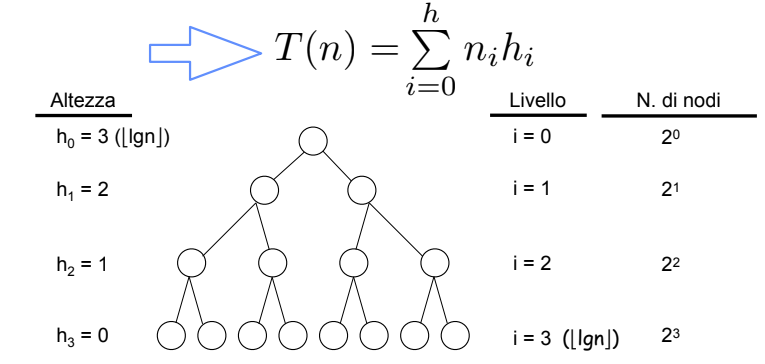
\includegraphics[scale=0.5]{img/costoHeap1.png}
    \end{figure}

    \begin{figure}[htbp]
        \center
        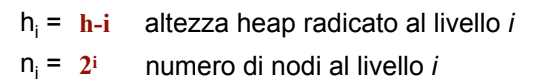
\includegraphics[scale=0.4]{img/costoHeap2.png}
    \end{figure}

    \begin{figure}[htbp]
        \center
        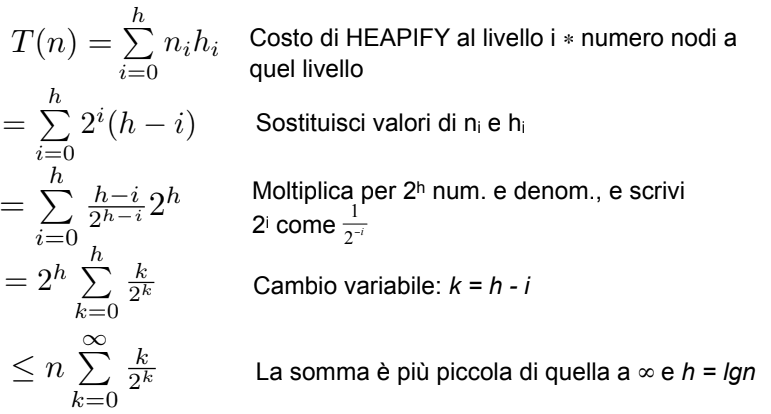
\includegraphics[scale=0.4]{img/costoHeap3.png}
    \end{figure}

Notiamo che il costo di $maxHeapify$ è proporzionale all'altezza del nodo nel quale lo si sta applicando. Dunque possiamo rendere generico il calcolo e, dopo vari passaggi algebrici e portando fuori $n$ dalla sommatoria, possiamo rifarci ad una serie notevole che converge. Dunque il costo di $buildMaxHeap$, applicando in bottom-up la funzione $maxHeapify$ avrà costo $O(n)$.
    
\end{enumerate}

\newpage

\subsubsection{Heapsort} L'Heapsort è un sort per confronti ottimale per tempo e spazio. A differenza dei sort visti fino ad ora infatti, è in place e ha costo $O(nlogn)$. Descriviamo il suo procedimento.

\begin{enumerate}
    \item Considerando come esempio un $maxHeap$, noi sappiamo che questo sarà implementato su array e la radice conterrà l'elemento massimo di tutto l'heap
    \item Possiamo dunque sostituire il primo elemento del vettore (\textbf{radice}) con l'ultimo
    \item Escludiamo con gli indici l'ultimo elemento dell'array
    \item Ricostituiamo un $maxHeap$ sui rimanenti elementi dell'array
    \item Reiterando questa procedura otterremo un array ordinato in senso crescente, dato che come proprietà abbiamo utilizzato quella del $maxHeap$
\end{enumerate}

    Ipotizziamo un array:

    \begin{equation}
        A=[7,4,3,1,2]
    \end{equation}
    
    \begin{figure}[htbp]
        \center
        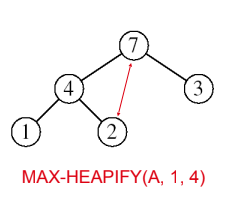
\includegraphics[scale=0.6]{img/heapSort2.png}
        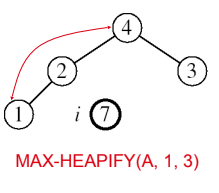
\includegraphics[scale=0.6]{img/heapSort3.png}
        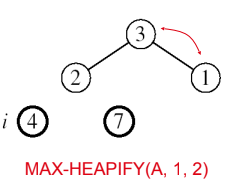
\includegraphics[scale=0.6]{img/heapSort4.png}
    \end{figure}

    \begin{figure}[htbp]
        \center
        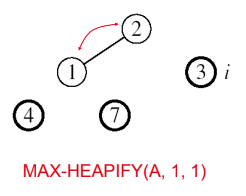
\includegraphics[scale=0.6]{img/heapSort5.png}
        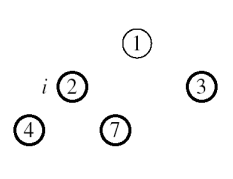
\includegraphics[scale=0.6]{img/heapSort6.png}
    \end{figure}

    Dunque, dopo l'applicazione dell'heapSort, l'array sarà:

    \begin{equation}
        A=[1,2,3,4,7]
    \end{equation}

\begin{lstlisting}[language=JavaScript]
heapSort(A){
	let tmp
	buildMaxHeap()
	for(i=A.length;i>0;i--){
		tmp=A[0]
		A[0]=A[i]
		A[i]=tmp
		maxHeapify(A,1)	
	}
}
\end{lstlisting}

\newpage

\subsection{Hashmap}

Una Hashmap è una struttura dati che per ogni chiave $k \in U$ universo delle chiavi, calcola il valore hash $h(k)$ che sarà la posizione nella tabella in cui sarà inserita la chiave $k$ stessa.

Prima però introduciamo un concetto simile ma più semplice:

\subsubsection{Tavole ad indirizzamento diretto} Se considerassimo un universo delle chiavi $U$ ragionevolmente piccolo, e un $m$ grandezza della tabella non troppo grande, allora potremmo discutere le operazioni effettuabili su questa struttura.

\begin{enumerate}
    \item Ricerca: Costo $\Theta(1)$
    
    \begin{lstlisting}[language=JavaScript]
    directAddressSearch(T,k)
    {
        return T[k]
    }
    \end{lstlisting}
    \item Inserimento: Costo $\Theta(1)$
    
    \begin{lstlisting}[language=JavaScript]
    directAddressInsert(T,x)
    {
        T[x.key]=x
    }
    \end{lstlisting}
    \item Cancellazione: Costo $\Theta(1)$
    
    \begin{lstlisting}[language=JavaScript]
    directAddressDelete(T,k)
    {
        T[x.key]=nil
    }
    \end{lstlisting}
\end{enumerate}

Questa pratica ha un ovvia debolezza: Se l'universo delle chiavi $U$ è troppo grande, sarebbe impossibile generare una tabella di dimensioni $|U|$. Dunque vogliamo una struttura che sia in grado di simulare queste prestazioni in tempo, ma che allo stesso tempo gestisca in maniera più attuabile lo spazio.

\newpage

\subsubsection{Funzione Hash}

\begin{figure}[htbp]
        \center
        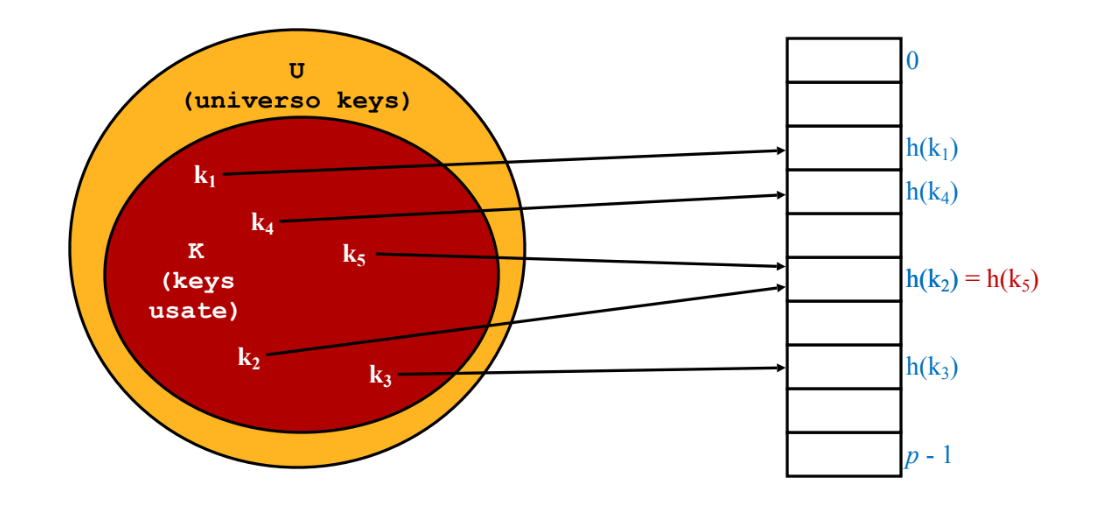
\includegraphics[scale=0.35]{img/hashMap1.png}
        \caption{Hashmap}
    \end{figure}

Notiamo gli elementi fondamentali elencandoli:

\begin{enumerate}
    \item $U$: universo delle chiavi
    \item $K$: insieme delle chiavi realmente utilizzate
    \item $h(k)$: funzione hash $h: U -> (0,1, ... ,m-1)$ che appunto, data una chiave $k \in U$ elabora il suo valore, calcolando la posizione nella quale verrà inserita nella tabella
    \item Tabella: Array di dimensione $m$
\end{enumerate}

\subsubsection{Collisione} Notiamo, nell'immagine 3, che il valore hash delle chiavi $k2$ e $k5$ è lo stesso. Dunque quelle due chiavi nella stessa posizione causeranno una collisione. Esistono diversi metodi per risolvere la collisione. Mostreremo \textbf{chaining} e \textbf{open addressing}.

\subsubsection{Chaining} Quando due chiavi $k_{i}$ e $k_{j}$ hanno lo stesso valore hash, allora l'ultimo dei due viene aggiunto in testa alla lista alla quale sta puntando la posizione $h(k_{i})=h(k_{j})$. Dunque gestiamo la collisione dando la possibilità di poter aggiungere più elementi in una sola posizione.

\begin{figure}[htbp]
        \center
        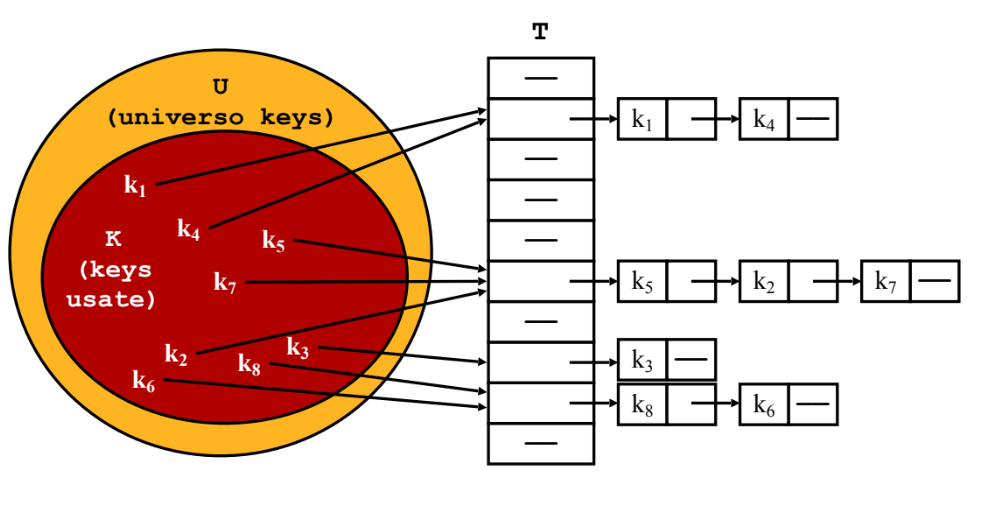
\includegraphics[scale=0.35]{img/hashMap2.png}
    \end{figure}

\newpage

\paragraph{Esempio di chaining} In questo caso, notiamo che stiamo considerando la tabella come array di liste concatenate. Dunque viene risolta la collisione tra chiavi.

\begin{figure}[htbp]
        \center
        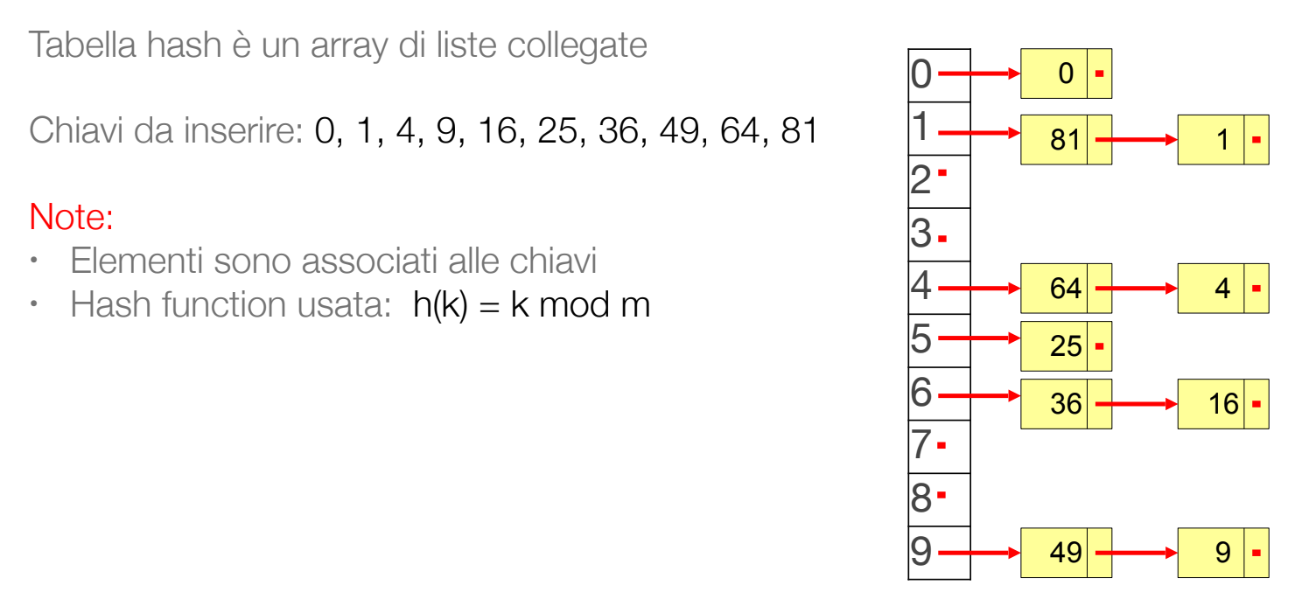
\includegraphics[scale=0.35]{img/chaining1.png}
    \end{figure}

\subsubsection{Operazioni e Costi - Chaining} Consideriamo le tre operazioni principali, ovvero $search(x)$, $delete(x)$ e $insert(x)$.

\paragraph{Load Factor} Il load factor è il rapporto tra $n$ numero di elementi nella tabella hash e $m$ grandezza della tabella.

\begin{equation}
    \lambda=\frac{n}{m}
\end{equation}

Rappresenta quindi la \textbf{media} di elementi contenuti in ogni posizione della tabella.

\paragraph{Caso peggiore del Chaining} Nella peggiore delle ipotesi, tutti i dati vengono inseriti in una sola posizione della tabella, dunque il costo della ricerca sarà $O(n)$ dato che sarà necessario scorrere la lista, sia in caso di successo che di insuccesso. 

\paragraph{Hashing uniforme semplice} E' necessario dunque assumere che ogni chiave ha la stessa probabilità di essere mappata in una delle posizioni della tabella.

\paragraph{Lunghezza media della lista} Dato che abbiamo affermato che $\lambda$ fosse equivalente alla media di elementi presenti in ogni posizione della tabella, allora assumiamo che la lunghezza della lista $T[h(k)] = \lambda$.

\paragraph{Costo Ricerca senza successo} Una volta aver assunto tutte le proprietà elencate sopra, analizziamo quali passi vengono eseguiti nel caso di una ricerca senza successo.

\begin{enumerate}
    \item Si accede alla lista, costo: $O(1)$
    \item La si scorre tutta, costo: $O(\lambda)$
\end{enumerate}

Dunque la \textbf{ricerca fallita} impiega tempo $\Theta(1+\lambda)$.

\newpage

\paragraph{Delete e Insert nel caso medio} Analizziamo anche queste due operazioni:

\begin{enumerate}
    \item Delete: Bisogna trovare l'elemento e rimuoverlo, dunque il costo sarà simile a quello della ricerca nel caso medio: $\Theta(1+\lambda)$. Nel caso di liste doppiamente collegate allora il costo sarebbe $O(1)$.
    \item Insert: L'inserimento costerà semplicemente $O(1)$ dato che aggiungeremo la chiave in testa alla nostra lista.
\end{enumerate}

\subsubsection{Funzioni Hash per interi}

Esempi di funzioni hash per interi, analizzandone le caratteristiche:

\paragraph{Division Method} Si sceglie questa funzione hash:

\begin{equation}
    h(k) = (k) mod (m)
\end{equation}

In genere è consigliato evitare determinati valori di m, infatti spesso si sceglie un m primo non troppo vicino ad una potenza di 2.

\paragraph{Multiplication Method} Ulteriore metodo per generare una funzione hash per interi:

\begin{enumerate}
    \item Si moltiplica la chiave $k$ per una costante $A$ e si sottrae la parte sua parte frazionaria
    \begin{equation}
        kA - partefrazionaria(ka)
    \end{equation}
    \item Si moltiplica questo valore per m e si prende il floor dell'espressione
    \begin{equation}
        h(k)=floor(m((kA)modulo1))
    \end{equation}
\end{enumerate}

\newpage

\subsubsection{Open Addressing} L'Open Addressing è un altro metodo che cerca di risolvere le problematiche causate dalla collisione di chiavi con stesso valore hash.

Ipotizzando dunque di voler inserire in una tabella $T$ una chiave $k2$ con lo stesso valore hash $h(k)$ di $k1$, l'Open Addressing gestirà questa collisione con il \textbf{probing}, ovvero avanzerà di $n$ posti nella tabella, dando un criterio a quella n in base al tipo di probing selezionato. Elenchiamo i tre tipi principali di probing:

\begin{enumerate}
    \item \textbf{Probing Lineare}: Il probing lineare è una tecnica che permette il controllo della posizione con indice $h(k)$ e in caso la posizione fosse piena, controlla in senso lineare le posizioni successive. I tentativi sono formalmente indicati come $f(i)$, dunque la funzione finale di hash $h(k)$ sarà la somma delle due funzioni $h^{'}(k)$ hash effettivo e $f(i)$, dunque:
    \begin{equation}
        h(k)=h^{'}(k)+f(i)
    \end{equation}

    \begin{figure}[htbp]
        \center
        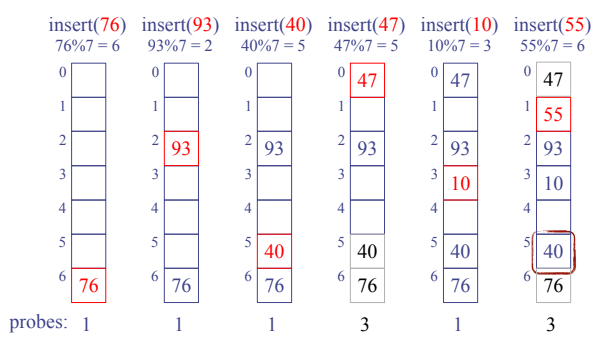
\includegraphics[scale=0.65]{img/probingLineare.png}
        \caption{Con probes indichiamo i correnti tentativi}
    \end{figure}

    Questa tecnica però soffre una conseguenza diretta della linearità proposta, ovvero il \textbf{clustering primario}. Pian piano infatti, ad ogni tentativo d'inserimento andremo a generare dei "blocchi" di dati che rallenteranno le operazioni, dato che saremo costretti a scorrerli tutti prima di poter trovare la posizione desiderata.

    \paragraph{Costo Ricerca fallita} Intuitivamente, si fa sempre il primo tentativo, e successivamente ti tenta con probabilità $\lambda$ il successivo, dunque il costo sarà:

    \begin{equation}
        \frac{1}{1-\lambda}
    \end{equation}
    
Dunque il probing rende bene se $\lambda \leq 0.5$. Ricordiamo che $\lambda$ rappresenta anche in questo caso il \textbf{load factor}.
Questo costo andrebbe però dimostrato formalmente*

\newpage

    \item \textbf{Probing Quadratico}: Simile al probing linare, semplicemente la funzione sommata che "skippava" elementi non sarà lineare ma quadratica. In formula:

    \begin{equation}
        f(i)=i^{2}
    \end{equation}
    
    \begin{equation}
        h(k)=h^{'}(k)+f(i)
    \end{equation}

Questo tipo di probing è quindi caratterizzato dal fatto che, considerando un indice $i$ di probing, invece di incrementarlo e tentare di nuovo, lo incrementa e considera la posizione al quadrato. Allo stesso modo del probing lineare, questo tipo di soluzione presenta la problematica del \textbf{clustering secondario}, che influenza meno negativamente la soluzione rispetto al tipo primario.

\item \textbf{Double Hashing}: La funzione sommata è un valore hash calcolato su una seconda funzione hash data. Dunque in formula:

\begin{equation}
    f(i)=i*h_{2}(k)
\end{equation}

\begin{equation}
    h(k)=h^{'}(k)+f(i)
\end{equation}

Per far in modo che la tabella venga utilizzata per intero, il valore $h_{2}(k)$ deve essere coprimo di $m$ che rappresenta la dimensione della tabella.
Due numeri sono coprimi se l'unico divisone che hanno in comune è 1.
    
\end{enumerate}

\begin{figure}[htbp]
        \center
        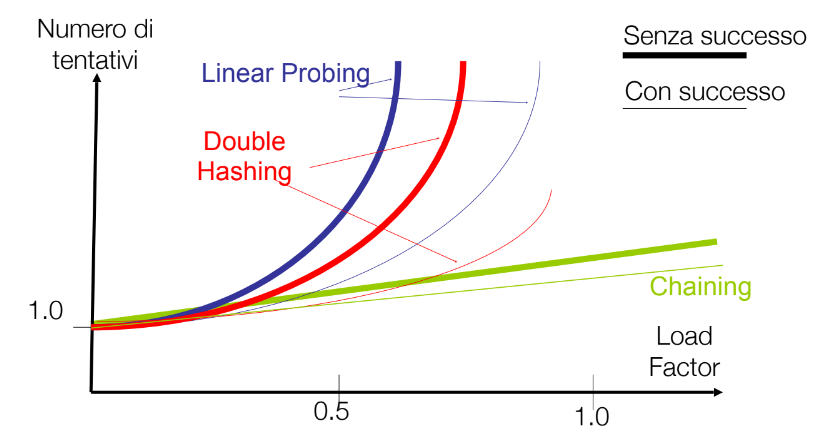
\includegraphics[scale=0.35]{img/openAddressingImg1.png}
    \end{figure}

    \begin{figure}[htbp]
        \center
        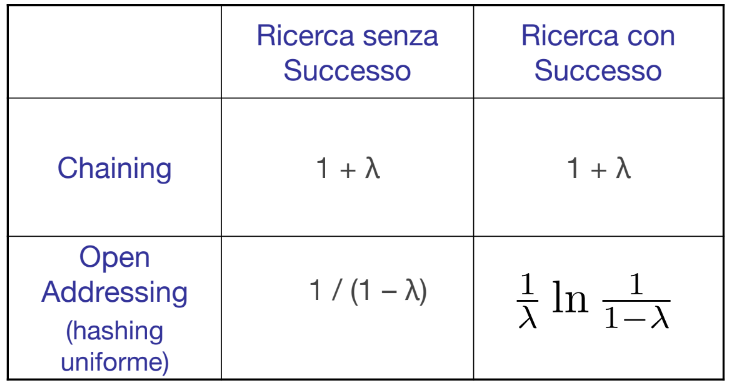
\includegraphics[scale=0.35]{img/openAddressingImg2.png}
        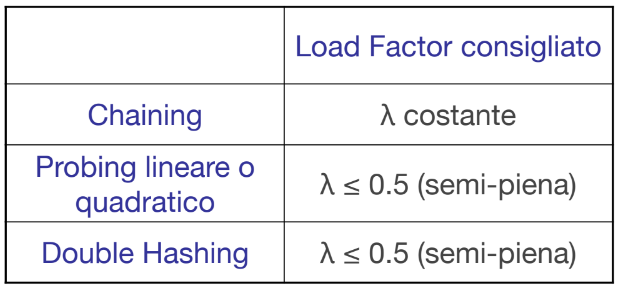
\includegraphics[scale=0.4]{img/openAddressingImg3.png}
    \end{figure}



\newpage

\section{Sorting Lineare}

In questo capitolo mostreremo dei tipi di sorting che ordinano in maniera differente dal 
confronto, e definiremo delle proprietà come la stabilità, analizzandone i costi.

\subsection{Counting Sort} Il Counting Sort è un tipo di ordinamento che non sfrutta i confronti, ma ipotizza che i dati inseriti siano interi contenuti nel range $[0,k]$. Dunque in questo modo non sarà necessario confrontare ogni dato con gli altri, infatti ogni numero contiene già la sua "posizione" dell'output ordinato.

Forniamo un esempio pratico per rendere più semplice l'applicazione del counting sort. Per implementare questo sort avremo bisogno di:

\begin{enumerate}
    \item A, array di input, dove $len=A.length$
    \begin{figure}[htbp]
        \center
        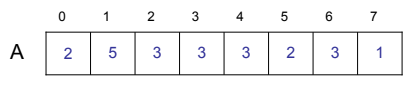
\includegraphics[scale=0.6]{img/countingSort1.png}
    \end{figure}
    \item B. array di output, che avrà la stessa $len$ di A
    \begin{figure}[htbp]
        \center
        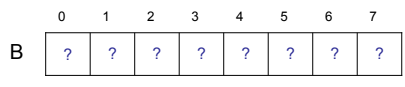
\includegraphics[scale=0.6]{img/countingSort2.png}
    \end{figure}
    \item C, array contatore, che ci permettera di conservare le occorrenze di ogni elemento nell'array
    \begin{figure}[htbp]
        \center
        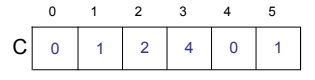
\includegraphics[scale=0.6]{img/countingSort3.png}
    \end{figure}
    \item k, range dove sono contenuti gli interi dell'array di input
    \begin{equation}
        k=5
    \end{equation}
\end{enumerate}

\paragraph{Perchè non utilizzare sempre il Counting Sort?} Questo tipo di sort dipende fortemente dal $K$ range su cui si distribuiscono i dati. Dunque in caso di cifre intere è molto vantaggioso, ma se stessimo lavorando su range più ampi non sarebbe per nulla vantaggioso.

\newpage

\begin{lstlisting}[language=JavaScript]
function countingSort(A,range)
{
    let C=[],B=[]
    //inizializzazione del contatore C
    for(let i=0;i<range;i++){
        C[i]=0
    }

    //conteggio occorrenze di elementi di A su contatore C
    for(i=0;i<A.length;i++){
        C[A[i]]++
    }

    //conteggio degli elementi minori o uguali
    for(i=1;i<range;i++){
        C[i]=C[i]+C[i-1]
    }

    //caricamento dell'array di output
    for(i=A.length;i>=0;i--){
        B[C[A[i]]]=A[i]
        C[A[i]]=C[A[i]]-1
    }

    return B
}
\end{lstlisting}

Questo tipo di sorting è detto \textbf{stabile} perchè, in caso di parità di valore, imposta l'ordine originale dell'array di input. Questo tipo di implementazione dunque mantiene un ordine tra gli elementi anche nelle varie iterazioni, questo torna utile nel caso di ordinamenti come il Radix Sort.

\subsection{Radix Sort} Il Radix Sort è un ordinamento che si basa sulla gestione delle cifre significative, dalla più piccola alla più grande. Quando ordiniamo ad esempio le unità non abbiamo nessuna particolare condizione da rispettare, ma passando ad esempio alle decine, dobbiamo tener conto dell'ordine generato dalla precedente iterazione in caso di decina dello stesso valore. Questo, espresso formalmente, vuol dire che necessità di un \textbf{ordinamento stabile}.

\begin{figure}[htbp]
        \center
        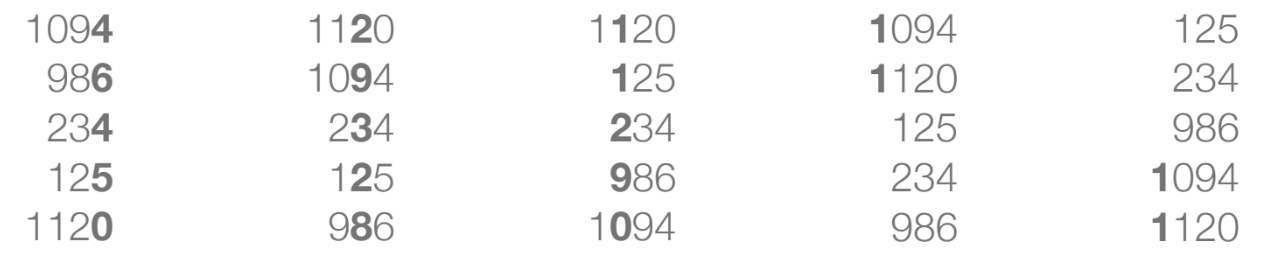
\includegraphics[scale=0.4]{img/radixSort1.png}
    \end{figure}

\newpage

\subsection{Ordinamento Stabile}

Fino ad ora abbiamo analizzato vari tipi di ordinamento, ma quali di questi mantengono, a parità di "chiave", l'ordine originale? $Merge Sort$, $Counting Sort$ e $Insertion Sort$ mantengono l'ordine originale a parità di chiave, dunque risultano \textbf{stabili}.

\begin{lstlisting}[language=JavaScript]
RadixSort(A, d)
{
    for (i=0; i < d; i++)
        StableSort(A) sulla cifra i
}
\end{lstlisting}

\section{Programmazione Dinamica}

La Programmazione Dinamica è un particolare paradigma che memorizza le soluzioni parziali su una \textbf{tabella di supporto}. Questo approccio è utilizzato solitamente per l'ottimizzazione di problemi.

\paragraph{Sottoproblemi ottimi ed dipendenza} Per poter utilizzare questo paradigma è necessario che il problema originale sia divisibile in \textbf{sottoproblemi comuni dipendenti}. Potremmo ad esempio menzionare la ricerca binaria in un array ordinato come controesempio: Quando in un array ordinato, decidiamo di esplorare il sottoarray destro o sinistro, queste due "partizioni" di problema originale sono del tutto indipendenti. Accade esattamente il contrario nel caso dell'approccio dinamico sui \textbf{Numeri di Fibonacci}.

\begin{figure}[htbp]
        \center
        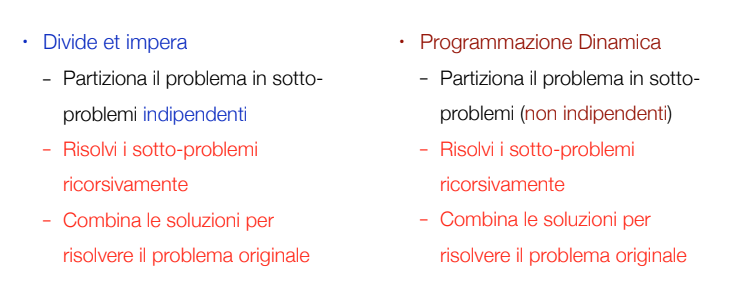
\includegraphics[scale=0.7]{img/ricVSdin.png}
    \end{figure}

\newpage

\subsection{Fibonacci}

\paragraph{Approccio Top-Down}

Analizziamo il costo di Fib ricorsivo, definendo semplicemente in pseudocodice le definizioni ricorsive e il caso base dei numeri di Fibonacci.

\begin{lstlisting}[language=JavaScript]
Fib( n ) { // n >= 0
    if (n <= 1)
        RETURN n;
    else
        RETURN Fib(n-1) + Fib(n-2);
}
\end{lstlisting}

\begin{figure}[htbp]
        \center
        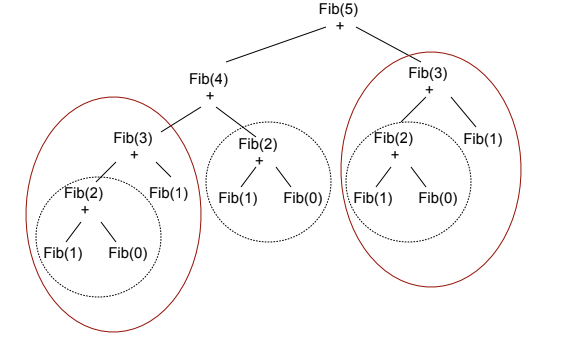
\includegraphics[scale=0.6]{img/fibRicorsivo.png}
    \end{figure}

Possiamo dunque notare i sottoproblemi comuni che sono cerchiati. Dunque svolgendo questo problema ricorsivamente andremo a sviluppare più volte calcoli che abbiamo già effettuato.

\paragraph{Approccio Bottom-Up} Proviamo ad eseguire lo stesso problema ma dalle foglie 

dell'albero alla radice, caricando ogni risultato in un array di supporto $F$.

\begin{lstlisting}[language=JavaScript]
Fib( n ) { // n >= 0
    F[0] = 0;
    F[1] = 1;
    for (k = 2; k <= n; k = k + 1)
        F[k] = F[k-1] + F[k-2];
    RETURN F[n];
}
\end{lstlisting}

\newpage

\subsection{Rod Cutting}

Definiamo il problema del taglio della corda, dove, avendo appunto una corda di una determinata lunghezza, e conoscendo i prezzi di ogni possibile taglio, dobbiamo determinare quale sia il modo migliore per tagliarla e venderla.

\paragraph{Brute Force} Il primo metodo che potrebbe essere pensato per un problema del genere è quello di considerare tutti i possibili tagli e ne prende il massimo. Costo di quest'operazione?

\begin{equation}
    O(2^{n-1})
\end{equation}

Vogliamo dunque trovare delle soluzioni che siano accessibili in termini di costo in tempo.

\paragraph{Ricorsione Top Down} Consideriamo la corda in questione, e consideriamo solo una prima parte, richiamando ricorsivamente la funzione sul resto della corda. 

\begin{equation}
    r_{n} = max \{ p_{i} + r_{n-1} : 1 \leq i \leq n \}
\end{equation}

\begin{figure}[htbp]
        \center
        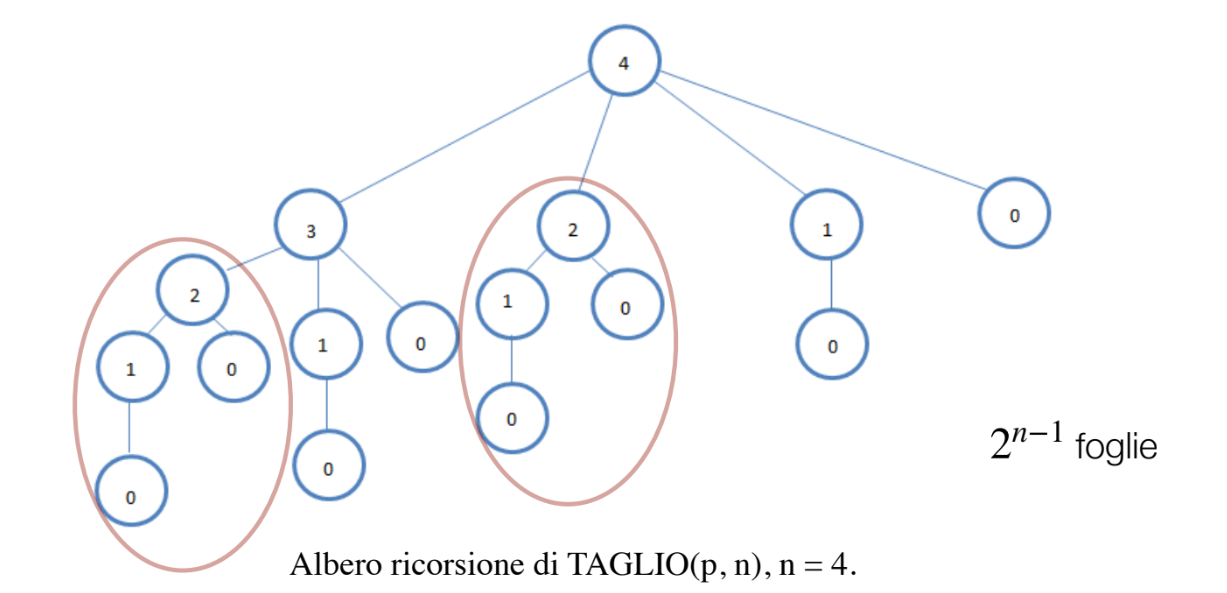
\includegraphics[scale=0.35]{img/rodCutting1.png}
    \end{figure}

Anche in questo caso però, notiamo dall'albero sviluppato che eseguiamo più volte gli stessi calcoli, rendendo molto meno efficiente questo algoritmo ricorsivo in top down. Perchè questo?. Perchè anche in questo caso, ad esempio, per una corda di lunghezza 3, stiamo "verificando" il costo migliore di ogni sua possibile composizione. Verificheremo quindi prima la corda lunga una unità con le possibilità restituite dal resto della corda, dato che verrà richiamata la funzione ricorsivamente sul resto. Costo di queste operazioni? $O(2^{n})$

\begin{figure}[htbp]
        \center
        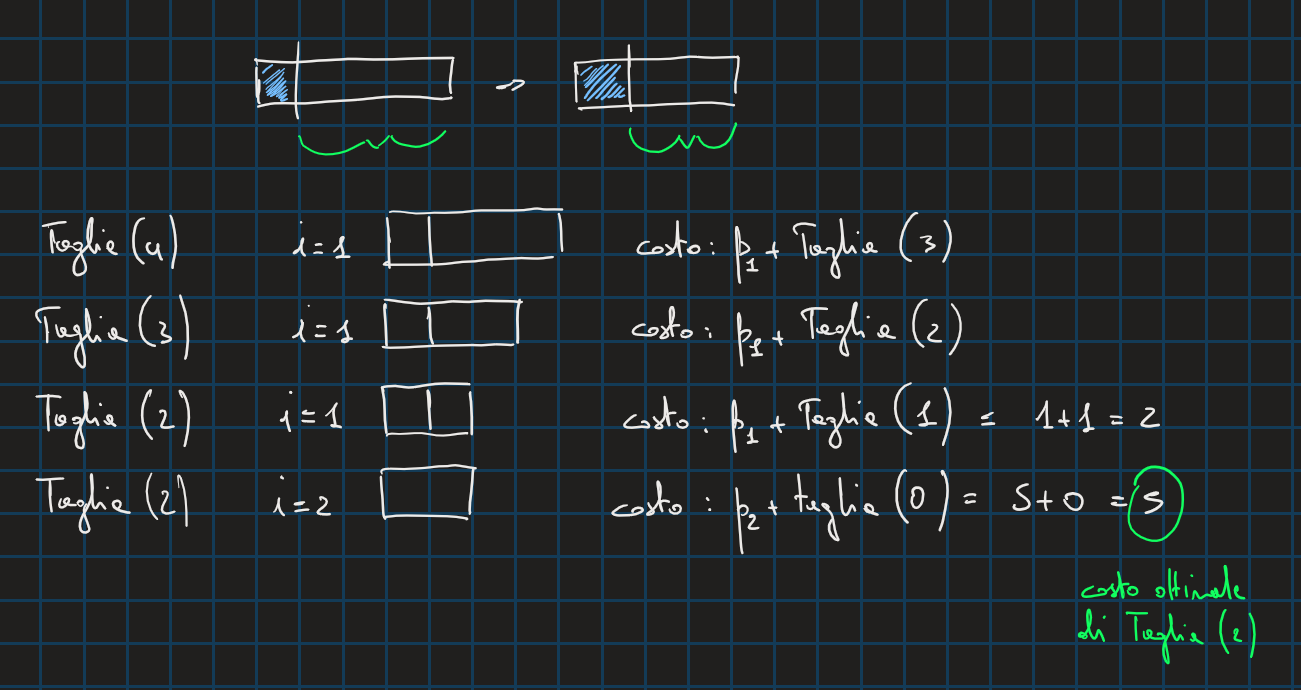
\includegraphics[scale=0.25]{img/rodCutting2.png}
    \end{figure}

\newpage

\paragraph{Soluzione Bottom Up} Come per Fibonacci, possiamo pensare di caricare una tabella che memorizzi i valori delle foglie dell'albero precedentemente rappresentato. Dunque consideriamo il massimo per ogni segmento, ma quando calcoleremo i sottosegmenti, sarà possibile accedere al loro miglior prezzo semplicemente accedendo alla tabella precedentemente caricata.

Definiamo gli elementi principali:

\begin{enumerate}

\item \textbf{Tabella $r$}

Definiamo la tabella $r$ dove l'indice sarà definito dalla lunghezza del sottosegmento e conterrà il costo ottimale di ogni possibile lunghezza dei sottosegmenti.

\begin{equation}
    r=[0,1,5,8,0]
\end{equation}

\item Definizione generale del problema di ottimizzazione

\begin{equation}
    r_{n} = max \{ p_{i} + r_{n-1} : 1 \leq i \leq n \}
\end{equation}

\item Pseudocodice dell'approccio in bottom up

\begin{lstlisting}[language=JavaScript]
TAGLIO-Dinamico(p,n)
    r[0..n]
    r[0]=0
    for j=1 to n
        q= -Infinity
        for i=1 to j
            if (q < p[i]+r[j-i]
                q= p[i]+r[j-i]
        r[j]=q
    return r
\end{lstlisting}

\item Esempio di istanza della soluzione

\begin{figure}[htbp]
        \center
        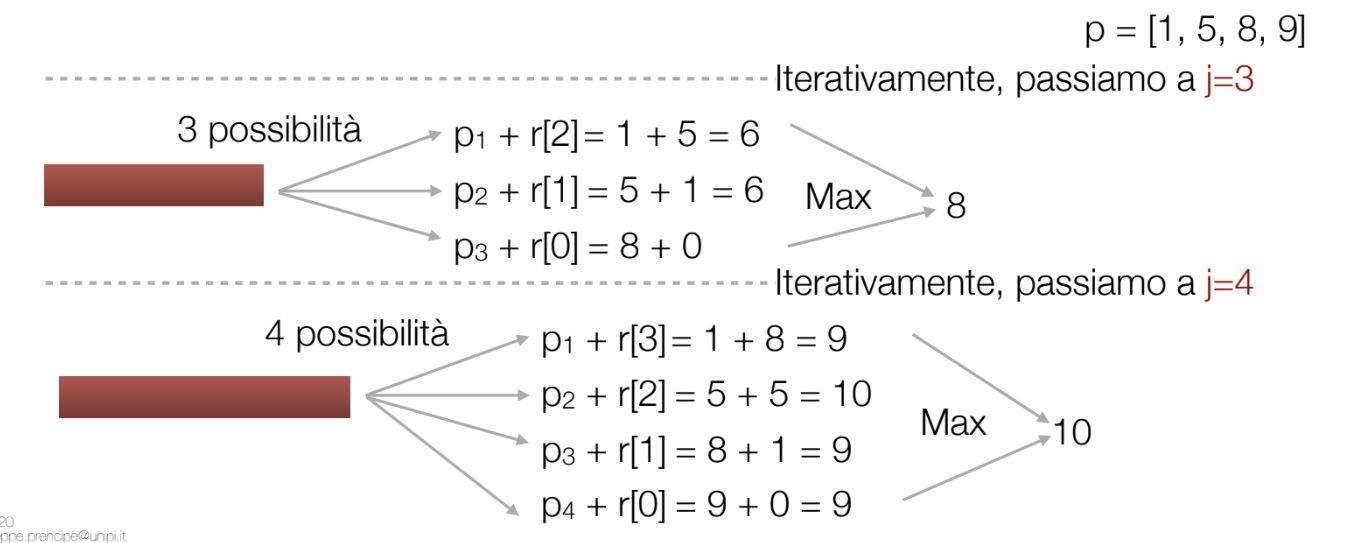
\includegraphics[scale=0.35]{img/rodCutting3.png}
    \end{figure}

\end{enumerate}

Il tempo dunque richiesto passerà da esponenziale a lineare, sacrificando lo spazio dedicato alla tabella di appoggio. Costi?

$O(n)$ in tempo e $O(m)$ in spazio ipotizzando $m$ come grandezza della tabella d'appoggio.

\newpage

\subsection{LCS} Con LCS intendiamo \(Longest Common Subsequence\), dunque considerando due stringhe in input consideriamo la sottosequenza comune (non consecutiva) tra le due. Dunque, analogamente ai problemi analizzati precedentemente ci saranno vari metodi proposti, come \(brute force\) e $Ricorsione \; Top Down$ e successivamente verrano elencati i vantaggi e le caratteristiche dell'approccio della $Programmazione$ $dinamica$.

\paragraph{Brute Force} Date due sequenze in input $A$ e $B$, allora

\begin{equation}
    LCS(A,B) = L(m,n) \; \; \; m = |A| \; \; \; e \; \; \; n = |B|
\end{equation}

Dunque si controlla se ogni sottosequenza in A sia o meno sottosequenza in B.

Bisogna però controllare tutte le sottosequenze, si impiega dunque tempo $O(n2^{m})$.

\paragraph{Ricorsione Top Down} Con la ricorsione Top Down possiamo considerare i prefissi delle sequenze stesse, dunque definiamo e commentiamo la ricorsione formale:

    \begin{figure}[htbp]
        \center
        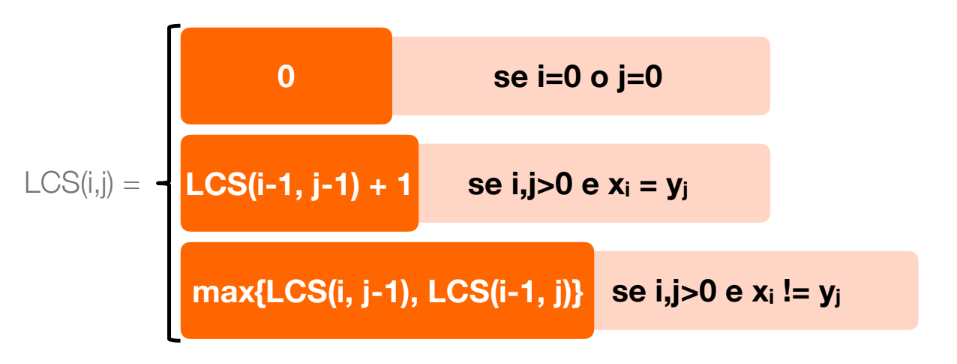
\includegraphics[scale=0.45]{img/LCS1.png}
    \end{figure}

\begin{enumerate}
    \item Caso Base: Gli indice sono entrambi a 0
    \item Primo Caso Ricorsivo: Gli indici sono entrambi superiori a 0 e i due caratteri delle sottosequenze correnti sono uguali, allora l'$LCS$ viene incrementata e entrambi gli indici vengono spostati verso sinistra.
    \item Secondo Caso Ricorsivo: Si prende il massimo delle due chiamate ricorsive a LCS scorrendo solo la prima verso sinistra o solo la seconda verso sinistra.
\end{enumerate}

Siamo dunque riusciti a trovare dei sottoproblemi dipendenti. Dunque impostiamo il calcolo con tabella di Programmazione Dinamica. In questo caso sarà una matrice.

\newpage

\paragraph{Calcolo Bottom Up}

Dedichiamo a questo calcolo una matrice di dimensione $nxm$. Analizziamo la definizione ricorsiva formale e le operazioni che esegue di conseguenza sulla matrice

\begin{figure}[htbp]
        \center
        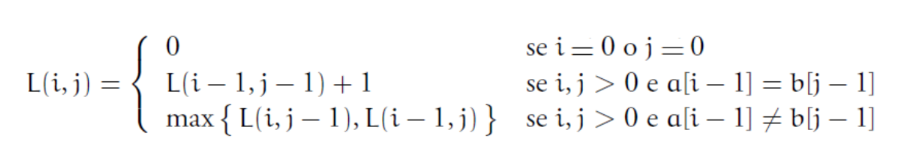
\includegraphics[scale=0.45]{img/LCS2.png}
        \includegraphics[scale=0.45]{img/LCS3.png}
\end{figure}

Ipotizzando di essere nella cella rossa, e di dover inserire un valore, avremo due possibilità:

\begin{enumerate}
    \item Se i due caratteri analizzati coincidono, si inserisce il valore della cella blu, posizionata in alto a destra rispetto alla corrente, incrementando il suo valore di 1.
    \item Se i due caratteri analizzati sono diversi, si inserisce il massimo tra le due caselle rappresentate in giallo.
\end{enumerate}

Dunque questa rappresenta l'interpretazione informale della sopraccitata definizione ricorsiva formale, dove abbiamo omesso il caso base che permette l'impostazione di prima riga e prima colonna a 0.

\paragraph{Esempio d'applicazione} Mostriamo un esempio pratico con due stringhe e relativa sottosequenza comune più lunga.

\begin{equation}
    S_{1}: \; <A,B,C,B,D,A> \; \; \; S_{2}: \; <B,D,C,A,B,A> 
\end{equation}

\begin{figure}[htbp]
        \center
        \includegraphics[scale=0.4]{img/LCS4.png}
\end{figure}

La lunghezza dell'$LCS$ sarà nella casella \(A[n]][m]\). Se volessimo ricostruire la sottosequenza in questione dovremmo seguire le frecce contrassegnate nella tabella, stampando il contenuto delle celle contrassegnate con una freccia diagonale.

\newpage

\subsection{Edit Distance} Vogliamo considerare la distanza massima tra due stringhe. Ci sono due possibili casi:

Consideriamo di poter inserire spazi allo scopo di allineare le sequenze 

\begin{enumerate}
    \item Caratteri uguali equivalgono a distanza 0
    \item Caratteri diversi, o carattere confrontato con spazio equivale a 1
\end{enumerate}

\paragraph{Formulazione Ricorsiva} Descriviamo il criterio del riempimento della matrice: 

\begin{figure}[htbp]
        \center
        \includegraphics[scale=0.4]{img/editDistance1.png}
        \includegraphics[scale=0.4]{img/editDistance2.png}
\end{figure}

Ipotizzando che la corrente casella analizzata sia quella in basso a destra tra quelle evidenziate, imposteremo il suo valore in questo modo:

\begin{enumerate}
    \item Se i due caratteri sono diversi si seleziona il minore tra i tre attorno alla corrente casella incrementandolo di 1
    \item Se i due caratteri sono uguali, il corrente viene settato come il valore della casella in diagonale rossa
\end{enumerate}

Ipotizzando due stringhe, e la tabella di Edit Distance completamente riempita seguendo la formulazione ricorsiva menzionata sopra, possiamo ricostruire anche il suo allineamento. Mostriamo un esempio commentato nella pagina successiva.

\newpage

\paragraph{Esercizio commentato su Edit Distance} 

Possiamo definire l'allineamento partendo dall'alto della matrice e "seguendo" le "frecce" che indicano quale casella ha provocato l'inserimento della successiva.

\begin{figure}[htbp]
        \center
        \includegraphics[scale=0.3]{img/esempioEditDistance.png}
\end{figure}

\begin{enumerate}
    \item \textbf{Freccia obliqua}: caratteri di riga e colonna vanno inseriti in entrambe le stringhe che stiamo producendo
    \item \textbf{Freccia orizzontale}: carattere della riga va inserito nella corrispondente stringa, mentre carattere della colonna non va inserito, sostituendolo con uno spazio
    \item \textbf{Freccia verticale}: carattere della colonna va inserito nella corrispondente stringa, mentre carattere della riga non va inserito, sostituendolo con uno spazio
\end{enumerate}

Una volta effettuati i passaggi raggiungendo l'ultima casella della matrice in basso a destra, possiamo definire che due caratteri diversi (o carattere spazio), confrontando le due stringhe prodotte, incrementeranno la distanza di edit di 1, mentre caratteri uguali non la incrementano.

\newpage

\subsection{Zaino 0-1} Il problema dello \textbf{zaino intero} è un esempio di approccio alla programmazione dinamica. Questo è differente dai problemi già mostrati, dato che è il primo che non si rifà ai sottoproblemi precedenti in maniera diretta. Introduciamo il problema:

\begin{figure}[htbp]
        \center
        \includegraphics[scale=0.4]{img/zaino1.png}
\end{figure}

\paragraph{Caratteristiche del problema} Abbiamo uno zaino che può accogliere degli oggetti, con un limite di capienza in peso. Dati dunque degli oggetti con valore e peso caratteristici, l'obiettivo sarà quello di massimizzare il valore contenuto nello zaino.

\begin{figure}[htbp]
        \center
        \includegraphics[scale=0.35]{img/zaino2.png}
\end{figure}

In questa immagine mostriamo come, la soluzione indicata con $S_{3}$
indica l'insieme ottimo di tre elementi in quanto a massimizzazione di valore. Dunque definiremo $S_{3}$ come soluzione ottima a 3 elementi. Notiamo però che $S_{4}$ oppure un generico $S_{k+1}$ potrebbe non contenere la precedente soluzione. Infatti, tenendo sempre la massimizzazione del valore come obiettivo, si nota che rimuovendo $I_{3}$ da $S$ ed aggiungendo $I_{4}$ otterremo la soluzione ottima per 4, dunque $S_{4}$

\paragraph{Sintesi} La soluzione ottima in $S_{k+1}$ potrebbe non contenere la sua diretta precedente sottosoluzione $S_{k}$

\paragraph{Forza Bruta} La soluzione in forza bruta del problema dello zaino intero porterebbe ad una complessità $2^{n}$, dato che sarebbe necessario controllare tutte le possibili composizioni. Proviamo ad ottimizzare questo costo.

\newpage

\paragraph{Definizione Ricorsiva}:

\begin{figure}[htbp]
        \center
        \includegraphics[scale=0.4]{img/zaino3.png}
\end{figure}

La definizione ricorsiva si divide dunque in due casi:

\begin{enumerate}
    \item Il peso dell'oggetto è maggiore del peso complessivo trasportabile, dunque considero i k-esimi meno uno elementi, ovvero gli elementi presenti senza il corrente.
    \item Cerco il massimo tra la composizione senza il corrente e la composizione più il corrente, rimuovendo un elemento dello stesso peso del corrente.
\end{enumerate}

\begin{figure}[htbp]
        \center
        \includegraphics[scale=0.35]{img/zaino4.png}
\end{figure}

\paragraph{Esempio d'istanza del problema} Mostriamo un istanza del problema Zaino 0-1 su matrice, dati quattro oggetti con (peso,valore)
$(2,3) \: (3,4) \: (4,5) \: (5,6)$

\begin{figure}[htbp]
        \center
        \includegraphics[scale=0.5]{img/zaino5.png}
\end{figure}

La tabella va letta in questa maniera: La riga indica quanti possibili elementi \textbf{in ordine} stiamo considerando nella combinazione. Il peso invece indica quanto può occupare la combinazione considerata. Dunque, facendo degli esempi:

\begin{enumerate}
    \item Riga 1: Considero solo il primo elemento da peso 0 a 5
    \item Riga 2: Considero le combinazioni tra primo e secondo elemento da peso 0 a 5
    \item Riga 3: Considero le combinazioni tra primo, secondo e terzo elemento da peso 0 a 5...
\end{enumerate}

\newpage

\paragraph{Analisi del costo - Zaino 0-1 e Programmazione Dinamica} Il costo dell'approccio dinamico per questo problema sarà $O(n*W)$, definita come \textbf{pseudo-polinomiale}. Perchè pseudo? Perchè per la prima volta non stiamo considerando solo il numero di elementi, ma anche una loro qualità, in questo caso il peso. Sarà dunque necessario valutare quanti bit saranno necessari per rappresentare il peso in questione.

\begin{figure}[htbp]
        \center
        \includegraphics[scale=0.3]{img/zaino6.png}
\end{figure}

In questa figura infatti mostriamo come potrebbe diventare persino esponenziale rispetto a $k$, ovvero i bit necessari per rappresentare il peso in questione.

\subsection{Greedy}

Con Greedy intendiamo una strategia basata sull'ottimo locale, nella speranza che coincida con l'ottimo globale. Non sempre infatti la strategia Greedy coincide con l'ottimo globale della soluzione, ma lo farà negli esempi proposti, dunque \textbf{Zaino Frazionario} e \textbf{Scheduling di Attività}

\subsubsection{Zaino Frazionario} Mostriamo l'esempio della strategia Greedy sulla versione frazionaria dello zaino. Consideriamo dunque il rapporto costo/peso delle frazioni in questione, dando priorità a questo durante il riempimento dello zaino con le varie frazioni.

\begin{figure}[htbp]
        \center
        \includegraphics[scale=0.5]{img/greedy1.png}
        \includegraphics[scale=0.5]{img/greedy2.png}
\end{figure}

\newpage

\paragraph{Simulazione selezione oggetti e costi} Dato dunque il rapporto costo peso, stabiliamo un ordinamento tra gli oggetti dati su questo criterio e selezioniamo man mano in ordine decrescente gli oggetti dal rapporto maggiore a quello minore. Stiamo dunque dando priorità al massimo corrente. Dunque i costi saranno $\Theta(n)$ se gli oggetti sono già ordinati in base al rapporto dato, altrimenti il costo corrisponderà a $\Theta(nlgn)$.

\subsubsection{Scheduling di attività} Lo scheduling di attività si pone come ottimo esempio per l'applicazione di una strategia Greedy. Assumiamo che, dato un insieme di attività, il nostro obiettivo sarà quello di determinare la combinazione che ci permetta di inserire quante più attività possibili.

Tutto l'algoritmo della scelta in Greedy dello scheduling si basa su questi passi:

\begin{enumerate}
    \item Scelgo un attività da cui cominciare
    \item Scarto tutte le attività il cui inizio è compreso nell'intervallo della prima attività (scarto le attività incompatibili)
    \item Scelgo tra le rimanenti l'attività che finisce prima tra le attività compatibili (applicazione della strategia Greedy)
    \item Reitero il procedimento fino alla conclusione di attività
\end{enumerate}

\begin{figure}[htbp]
        \center
        \includegraphics[scale=0.5]{img/greedy3.png}
\end{figure}

Dato questo esempio, è necessario stabilire \textbf{quando} la strategia Greedy porta alla soluzione ottima globale.

\newpage

\subsubsection{Dimostrazione Soluzione Ottima del Greedy} Per dimostrare che una soluzione greedy sia ottima anche globalmente è necessario dimostrare:

\begin{enumerate}
    \item Il problema ha una \textbf{sotto-struttura ottima}, dunque possiamo approcciare il sotto-problema in maniera simile
    \item Viene soddisfatta la \textbf{greedy-choice property}, ovvero
    \begin{enumerate}
        \item Dimostrare che il greedy porta alla soluzione ottima
        \item Soluzione greedy che procede in \textbf{top-down}
    \end{enumerate}
\end{enumerate}

\paragraph{Dimostrazione di esistenza soluzione ottima} Dimostriamo che il Greedy coincide con la soluzione ottima, 
\subparagraph{Elementi Fondamentali}
\begin{enumerate}
    \item $A$ soluzione ottima
    \item $S$ insieme di attività da schedulare
    \item $a_{1}$ scelta Greedy
    \item $a_{k}$ primo elemento dell'ottimo $A$
\end{enumerate}

\subparagraph{Confronto di primo elemento e Scelta Greedy}

\begin{enumerate}
    \item Dato $A$, il suo primo elemento sarà $a_k$, e la scelta effettuata dal Greedy sarà $a_{1}$. Abbiamo due possibilità:
    \begin{enumerate}
        \item $a_{1} = a_{k}$ Scelta Greedy coincide con primo elemento di $A$ ottimo.
        \item Scelgo una nuova soluzione $B$, dato che $fine$ di $a_{1}$ è minore o uguale a $fine$ di $a_{k}$, allora sostituiamo $a_{k}$ con $a_{1}$. Notiamo che il numero di attività in $B$ coincide con il numero di attività in $A$. Dunque anche $B$ è ottimo, dato che l'obiettivo corrente è quello di massimizzare il numero di attività.
    \end{enumerate}
\end{enumerate}

\subparagraph{Resto degli elementi e induzione}

\begin{enumerate}
    \item Se $A$ è ottimo per $S$, allora $A^{'}$ sarà ottimo per $S_{'}$, dove $S_{'}$ è l'insieme degli elementi appartenenti ad $S$ tali che ogni tempo d'inizio delle attività in $S_{'}$ sia successivo alla fine dell'attività $a_{1}$.
    \item La validità in questo contesto di $S_{'}$ è dimostrabile per assurdo, dato che estendendo un ipotetico $B_{'}$ ed aggiungendo ad esso l'attività $a_{1}$ avremmo generato una soluzione $B$ per $S$ più grande dell'ottimo $A$.
\end{enumerate}

\newpage

\section{Grafi} Definiamo un grafo come una coppia $G = (V,E)$, dove $V$ è l'insieme dei vertici e $E$ l'insieme degli archi.

\subsection{Definizioni e caratteristiche}

\paragraph{Grafo Denso/Sparso} Un grafo è detto:

\begin{enumerate}
    \item Sparso : $|E| \approx |V|$
    \item Denso : $|E| \approx |V|^{2}$
\end{enumerate}

Ricordiamo anche che il massimo numero di archi per un grafo è $|V|^{2}$.

\paragraph{Componente connessa}

Presi due nodi $v,u$ questi fanno parte della stessa componente connessa se sono raggiungibili con un cammino da $v$ a $u$.

\paragraph{Self-Loop/Cappio} In un grafo orientato, un arco che va da un generico nodo $u$ a $u$ è definito Self-Loop.

\paragraph{Rappresentazione in matrice di adiacenza} Un grafo potrebbe utilizzare come supporto di memorizzazione una matrice che utilizza come indici gli stessi nodi e pone $1$ nella cella corrispondente ad un arco esistente e $0$ dove non esiste un arco tra i nodi presi in considerazione.

\begin{figure}[htbp]
        \center
        \includegraphics[scale=0.55]{img/matriceGrafo.png}
\end{figure}

Questo è solo un tipo di possibile supporto di memorizzazione per i grafi. Questi ultimi infatti potrebbero essere memorizzati con liste di adiacenza.

\paragraph{Grafo Pesato} Un grafo pesato associa ad ogni arco un elemento. Solitamente questi elementi sono interi, dato che diamo per scontato che esista un algebra ed un ordinamento su questi ultimi. Ma stabilendo queste due caratteristiche su altri oggetti, potremmo associare ad ogni arco una qualsiasi etichetta, non solo numeri.

\paragraph{Cammino} Un cammino è un insieme di nodi connessi, tali che partendo da un nodo $v$ è possibile raggiungero il nodo $u$.

\paragraph{Spanning Tree} Uno Spanning Tree, detto anche Albero di Copertura, è un albero che "certifica" la connessione tra nodi. Dunque rappresenta l'albero minimo di connessione tra i nodi di un grafo.

\newpage



\subsection{Attraversamento di Grafo}

Definiamo l'attraversamento di un grafo $G = (V,E)$ con vertice $s \in V$ detto $sorgente$ l'esplorazione di ogni vertice raggiungibile nel grafo dal vertice $s$.

\begin{figure}[htbp]
        \center
        \includegraphics[scale=0.55]{img/attraversamentoGrafo.png}
        \caption{In questo caso la sorgente è il nodo C, F è l'unico nodo non raggiungibile dalla sorgente}
\end{figure}

\paragraph{Shortest Path} Dati due nodi $u,v$, uno shortest path è un cammino minimo (contenente il numero minimo di archi) tra i due nodi. Solitamente, contestualizzato all'attraversamento di grafi, uno dei due nodi è settato alla sorgente. Ricordiamo che i cammini minimi in un grafo non sono unici, ma potrebbero esisterne diversi. 

\paragraph{Distanza dalla sorgente} I cammini minimi tengono considerazione solo del numero di archi tra i due nodi in questione, $\delta(s,v)$ come distanza tra la sorgente ed un nodo dato.

\subsubsection{BFS - Breadth First Search} La BFS è la visita in ampiezza di un grafo. Questo tipo di visita sfrutta come struttura dati di supporto una \textbf{coda}. Viene dunque messa in coda la sorgente da cui si parte e successivamente si valuta, aggiungendo il suo vicinato . Dunque "valutare" corrisponde ad inserire in coda il vicinato di un nodo. Ricordiamo che il vicinato di un nodo è l'insieme di nodi a cui è connesso il nodo in questione.

\paragraph{Versione 1/Versione 2}

Facendo riferimento alle slide del corso, vengono mostrati due diversi modi di implementare la BFS. La prima tra queste implementazioni non gestiva il caso in cui fosse presente un ciclo nel grafo. Dunque si implementa la seconda versione che grazie alla gestione "a colori" permette di valutare lo stato di un nodo:

\begin{enumerate}
    \item Colore Bianco: Il nodo in questione non è mai stato inserito in coda, quindi non è mai stato visitato.
    \item Colore Grigio: Il nodo in questione è stato inserito in coda, ma ancora non è stato valutato.
    \item Colore Nero: Il nodo è stato inserito in coda ed è stato anche rimosso dalla coda stessa essendo stato valutato.
\end{enumerate}

\newpage

\paragraph{Analisi del costo in tempo} Analizziamo il costo dell'algoritmo proposto nelle slide.

Il costo in tempo è scandito dalla visita delle liste di adiacenza che stiamo ipotizzando come tipo di memorizzazione del grafo. Per ogni vertice, bisogna valutare tutta la relativa lista di adiacenza, dunque la lista visiterà al massimo ogni arco, è scandita una sola volta ogni lista di adiacenza. E lo farò per ogni nodo. Dunque il costo sarà: 
\[O(|V|+|E|)\]

\paragraph{Analisi del costo in spazio} Dobbiamo memorizzare tutti i nodi, e la coda, nella peggiore delle ipotesi, dovrà mantenere tutti i nodi, e non può crescere più del numero di nodi stesso. Dunque lo spazio sarà:

\begin{equation}
    O(|V|)
\end{equation}

\paragraph{Shortest Path Distance e BFS} Considerando un generico nodo $v$ e la sorgente $s$, la BFS permette il calcolo della distanza minima tra $v$ ed $s$, come $\delta(s,v)$. Questo si basa sulla proprietà tale che dato $(u,v)$

\begin{equation}
    \delta(s,v) \leq \delta(s,u) + 1 
\end{equation}

\begin{figure}[htbp]
        \center
        \includegraphics[scale=0.55]{img/BFS1.png}
\end{figure}

Dunque la gestione del minimo numero di archi tra sorgente e nodo è di natura induttiva.

\paragraph{Caratteristiche BFS}

\begin{enumerate}
    \item Trova il cammino di lunghezza minima
    \item In grafi non pesati, trova il costo ottimo
    \item In grafi pesati, non trova il costo ottimo
\end{enumerate}

\newpage

\paragraph{BFS e relativo Spanning Tree} 

Abbiamo definito uno Spanning Tree come un albero che certificava la connessione tra nodi. La BFS permette la costruzione di uno Spanning Tree su un grafo, scegliendo tra i possibili shortest path sul criterio della visita in ampiezza.

\begin{figure}[htbp]
        \center
        \includegraphics[scale=0.5]{img/BFS2.png}
\end{figure}

\paragraph{Sottografo dei predecessori}

Sottografo che certifica la connessione definito su sottoinsiemi di vertici e archi.

\begin{figure}[htbp]
        \center
        \includegraphics[scale=0.5]{img/BFS3.png}
\end{figure}

Gli archi del sottografo sono detti $tree \: edges$. Dunque ogni nodo, tranne la sorgente avrà esattamente un predecessore.

\paragraph{Operazioni su BFS} Alcune operazioni, come la stampa degli shortest path, data la sorgente $s$ e un nodo generico $v$, si basa sull'albero prodotto dalla BFS, e visitando i nodi richiesti. Dunque molte operazioni simili si basano sull'utilizzo dei dati calcolati durante la costruzione dell'albero minimo.

\newpage

\subsubsection{DFS - Depth First Search}

La DFS è la visita in profondità di un grafo. Questo tipo di visita sfrutta come struttura dati una \textbf{pila}. Viene naturale implementare ricorsivamente questo tipo di visita data la pila dei record di attivazione della funzione ricorsiva in questione che gestirebbe automaticamente la struttura dati.

\begin{figure}[htbp]
        \center
        \includegraphics[scale=0.4]{img/DFS1.png}
\end{figure}

\paragraph{Visita in DFS e tipi di archi}

La DFS presenta quattro possibili tipi di archi:

\begin{figure}[htbp]
        \center
        \includegraphics[scale=0.55]{img/DFS2.png}
\end{figure}

\begin{figure}[htbp]
        \center
        \includegraphics[scale=0.55]{img/DFS3.png}
\end{figure}

Queste classificazioni degli archi nella DFS permette una visualizzazione grafica dei casi previsti dal $Parenthesis \: Theorem$ che formalizza il concetto che sta dietro al "colore" dei vertici, sfruttando degli intervalli.

\newpage

\paragraph{Parenthesis Theorem} Per ogni $u,v$, indichiamo

\begin{enumerate}
    \item $d[u] \: \: - \: \: f[u] $ l'intervallo del nodo $u$.
    \item $d[v] \: \: - \: \: f[v] $ l'intervallo del nodo $v$.
\end{enumerate}

Dovrà dunque essere valida esattamente una tra queste condizioni:

\vskip 1cm

\begin{enumerate}
    \item Gli intervalli $d[u] \: \: - \: \: f[u] $ e $d[v] \: \: - \: \: f[v] $ sono \textbf{completamente disgiunti}, che corrisponde al fatto che nè $u$ nè $v$ sono discendenti uno dell'altro.

    \begin{figure}[htbp]
        \center
        \includegraphics[scale=0.55]{img/parenthesis1.png}
    \end{figure}

    \vskip 2cm
    
    \item L'intervallo $d[u] \: \: - \: \: f[u]$ è \textbf{completamente contenuto} nell'intervallo $d[v] \: \: - \: \: f[v]$, dunque $u$ è discendente di $v$.

    \begin{figure}[htbp]
        \center
        \includegraphics[scale=0.35]{img/parenthesis3.png}
    \end{figure}

    \vskip 2cm
    
    \item L'intervallo $d[v] \: \: - \: \: f[v]$ è \textbf{completamente contenuto} nell'intervallo $d[u] \: \: - \: \: f[u]$, dunque $v$ è discendente di $u$.

    \begin{figure}[htbp]
        \center
        \includegraphics[scale=0.35]{img/parenthesis2.png}
    \end{figure}
    
\end{enumerate}

\newpage

\subsubsection{Topological Sort}

Un ordinamento topologico è un esempio di ordinamento che risolve delle \textbf{dipendenze} tra elementi. Possiamo dunque estrapolare un possibile ordinamento topologico da un grafo grazie all'utilizzo di una \textbf{DFS} e di una \textbf{PILA}. E' però necessaria una specifica condizione, ovvero:

\begin{enumerate}
    \item Esiste un Ordinamento Topologico $\Leftrightarrow$ il Grafo è un DAG
\end{enumerate}

L'obiettivo dell'ordinamento topologico è dunque quello di stabilire se esiste o meno "la dipendenza" tra gli elementi. A causa di questo non può essere presente un ciclo nel grafo, perchè staremmo affermando che $A$ dipende da $B$ e che contemporaneamente $B$ dipende da $A$. Questo non è possibile ed è definito come \textbf{deadlock}.

\paragraph{Implementazione con Pila e DFS}

Descriviamo l'algoritmo che implementa l'ordinamento topologico in passi:

\begin{enumerate}
    \item Eseguo un $DFS$ su grafo $G$, calcolando dunque i tempi di fine per ogni vertice $v$ rispetto ad una sorgente data
    \item Quando un vertice generico $v$ viene del tutto valutato viene inserito in una pila
    \item Restituisco la pila generata durante la valutazione di tutti i vertici
\end{enumerate}

Questa implementazione sfrutta dunque la proprietà $LIFO$ della pila per rappresentare uno dei possibili ordinamenti topologici dato un grafo.

\paragraph{Costo del Topological Sort} L'unica differenza tra queste operazioni ed una visita in $DFS$ è l'inserimento nella pila che costa $O(1)$, dunque asintoticamente costerà quanto la visita in $DFS$, quindi $O(|n|+|m|)$.

\begin{figure}[htbp]
        \center
        \includegraphics[scale=0.65]{img/ordinamentoTopologico1.png}
    \end{figure}

\newpage

\subsubsection{Algoritmo di Dijkstra}

L'Algoritmo di Dijkstra ha l'obiettivo di determinare un insieme $S$ in un grafo pesato, dove sono stati "salvati" i valori della distanza in peso di ogni nodo dalla sorgente $s$ data.

L'intero algoritmo si basa sull'utilizzo di una coda di priorità e dell'operazione

di $relaxation$. Descriviamo in passi l'algoritmo:

\begin{enumerate}
    \item \textbf{Inizializzazione}: Si setta la distanza dalla sorgente $s$ per ogni nodo del grafo $G$. Dunque ci sono due possibili casi:
    \begin{enumerate}
        \item \textbf{Il nodo corrisponde alla sorgente}: La sua distanza dalla sorgente sarà settata a 0.
        \item \textbf{Il nodo non corrisponde alla sorgente}: La sua distanza dalla sorgente sarà settata ad $\infty$.
    \end{enumerate}
    \item \textbf{Iterazione sulla Min Coda}: Si seleziona dalla coda l'elemento con distanza minore, e si rilassano gli adiacenti, iterando su questo criterio fino a quando la coda non è vuota. Dunque descrivendo dei passi generici:
    \begin{enumerate}
        \item Si seleziona il primo nodo con priorità maggiore nella coda, ovvero la sorgente, avendo distanza 0 dalla sorgente stessa.
        \item Selezionare vuol dire effettuare l'operazione di $relax$ sui nodi adiacenti, seguendo la priorità impostata dalla coda. Selezionare un nodo permette la sua rimozione dalla coda.
        \item L'operazione di $relax$ vuol dire verificare se la potenziale distanza attuale dalla sorgente è migliore di quella già associata al nodo stesso. Dunque si effettua uno scambio se la distanza nuova è più breve.
    \end{enumerate}
\end{enumerate}

\begin{lstlisting}[language=JavaScript]
Dijkstra(G, s) {
    Q = empty vertex priority queue;
    for each v in V {
        if (v == s) v.d = 0
        else v.d = infinity;
        v.p = nil;
        add v to Q with priority v.d;
    }
    while (Q != empty) {
        u = vertex with min priority in Q;
        for each v in u.adj {
            alt = u.d + weight(u,v);
            if (alt < v.d) {
                v.d = alt;
                v.p = u;
                decrease_priority(Q,v,alt)
            }
        }
    }
}
\end{lstlisting}

\newpage

\paragraph{Analisi del costo} Analizziamo il costo dell'algoritmo di Dijkstra implementato con coda di min priorità:

\begin{figure}[htbp]
        \center
        \includegraphics[scale=0.55]{img/dijkstra1.png}
    \end{figure}

Il costo finale dell'algoritmo sarà dunque

\begin{equation}
    O(|V|+|E|log(|V|))
\end{equation}

\paragraph{Commento su cicli di peso negativi} Questo algoritmo presenta un problema, si infrangerebbe infatti la proprietà \textbf{monotona} che permette l'accumulo e il calcolo di nuove distanze su quelle precedenti. Questo problema viene risolto nell'algoritmo proposto da Bellman Ford, a costo di una complessità in tempo maggiore.

\begin{figure}[htbp]
        \center
        \includegraphics[scale=0.45]{img/dijkstra2.png}
    \end{figure}

\newpage

\paragraph{Dimostrazione per Invariante}: Dimostriamo per invariante l'algoritmo di Dijkstra

Rendiamo nota la proprietà che vogliamo che sia rispettata alla fine dell'esecuzione dell'algoritmo stesso:

\vskip 1cm

\begin{equation}
    PROP1: \: \forall \: v \in V \: | \: v.d = \delta(s,v)
\end{equation}

\vskip 1cm

Dunque che ogni vertice $v$ abbia in $v.d$ la lunghezza dello shortest path da $s$ a $v$.

\begin{enumerate}
    \item \textbf{Inizializzazione}: $PROP1$ è valida nella sorgente, 
    assumendo che
\[\delta(s,s) = 0\]

\vskip 1cm

    \item \textbf{Mantenimento}:
    \begin{enumerate}
        \item Consideriamo un vertice visitato $u$ e uno non visitato $v$ con priorità massima, influirebbe in modo meno pesante possibile sulla somma
        \item Assumiamo allora che $v.d = u.d + weight(u,v)$
        \item Per dimostrare che la scelta del nodo $v$ sia la migliore effettuabile, scegliamo per assurdo un altro nodo che arrivi in maniera migliore a $v$, dunque un ipotetico nodo $z$ per assurdo. Allora abbiamo due sottocasi:
        \begin{enumerate}
            \item Se $z$ \textbf{non visitato}, $z.d > v.d$, allora abbiamo una contraddizione, dato che avevamo affermato che la scelta migliore sul peso sarebbe stata quella di $v$
            \item Se $z$ \textbf{visitato}, allora avremmo $v.d = z.d + weight(z,v)$, ma questo causa contraddizione dato che avevamo stabilito che $v.d = u.d + weight(u,v)$
        \end{enumerate}
    \end{enumerate} 

    \vskip 2cm

    
    \item \textbf{Conclusione}: Alla fine dell'algoritmo termina l'estrazione dalla coda, dunque non ha senso controllare ulteriori condizioni se non durante l'esecuzione stessa.
\end{enumerate}

\newpage

\subsubsection{Algoritmo di Bellman Ford}

Mostriamo il relativo pseudocodice e successivamente descriviamolo:
\begin{lstlisting}[language=JavaScript]
Bellman-Ford(G, s) {
    for each v in V {
        if (v == s) v.d = 0
        else v.d = infinity;
        v.p = nil;
    }
    for (i=1, i<|V|, i++) {
        for each (u,v) in E {
            alt = u.d + weight(u,v);
            if (alt < v.d) {
                v.d = alt;
                v.p = u;
            }
        }
    }
    for each (u,v) in E {
        if (v.d > u.d + weight(u,v)) 
            return false
    }
    return true
}
\end{lstlisting}

Questa implementazione ha lo scopo di ritornare $true$ se esiste nel grafo dato un \textbf{ciclo di peso negativo}, altrimenti ritorna $false$. Possiamo descrivere le sue parti fondamentali:

\vskip 2.5cm

\begin{enumerate}
    \item \textbf{Inizializzazione}: 
    \begin{lstlisting}[language=JavaScript]
for each v in V {
    if (v == s) v.d = 0
    else v.d = infinity;
    v.p = nil;
}
\end{lstlisting}
Si setta la distanza dalla sorgente di ogni nodo a $\infty$ e la sorgente stessa a 0.



\newpage
\vskip 2.5cm

\item \textbf{Ciclo e Rilassamento per ogni nodo}: 
    \begin{lstlisting}[language=JavaScript]
for (i=1, i<|V|, i++) {
    for each (u,v) in E {
        alt = u.d + weight(u,v);
        if (alt < v.d) {
            v.d = alt;
            v.p = u;
        }
    }
}
\end{lstlisting}
Per ogni nodo tranne la sorgente, si tenta il rilassamento calcolando $ALT$ ovvero la potenziale nuova distanza dalla radice per ogni arco del nodo selezionato. Se $ALT$ è migliore del corrente $v.d$ allora $v.d$ viene sostituito con $ALT$.
\vskip 2.5cm

\item \textbf{Controllo di cicli negativi}: 
\begin{lstlisting}[language=JavaScript]
for each (u,v) in E {
        if (v.d > u.d + weight(u,v)) 
            return false
    }
    return true
}
\end{lstlisting}
Controlla la presenza di cicli negativi all'interno del grafo, iterando su ogni arco.
\end{enumerate}

\newpage

\section{Complessità Computazionale}

Per introdurre l'argomento, è prima necessario stabilire quale sia il modello computazionale di riferimento attuale.

\subsection{Modelli Computazionali}

\paragraph{Modello RAM} L'astrazione dei moderni calcolatori è caratterizzata dalle seguenti caratteristiche:

\begin{enumerate}
    \item Ogni cella di memoria può contenere una quantità di dati finita.
    \item Impiega lo stesso tempo per accedere ad ogni cella di memoria.
    \item Le principali operazioni che può effettuare sono \textbf{lettura} e \textbf{scrittura} in 1 unità di tempo.
\end{enumerate}

\paragraph{Macchina di Turing} Potremmo rappresentare un modello computazionale alternativo che è però in grado di effettuare le stesse operazioni del modello \textbf{RAM} moderno:

\begin{figure}[htbp]
    \center
    \includegraphics[scale=0.45]{img/macchinaTuring.png}
\end{figure}

Questo modello si basa su una $testina$, un $processore$ ed un $programma$. In 1 unità di tempo può:
\begin{enumerate}
    \item Leggere o scrivere nella cella corrente
    \item Spostarsi (destra o sinistra) oppure rimanere fermo.
\end{enumerate}

Il punto di questa introduzione è quello di mostrare che modelli diversi possono effettuare simili operazioni. Dunque volendo discutere del tempo di esecuzione di un programma, sarebbe necessario considerare troppe variabili se non volessimo concentrarci solo sull'efficienza della soluzione proposta ma di un efficienza sistemica.

\subsection{Classi Computazionali}

In questa sezione analizzeremo non più la \textbf{complessità di algoritmi} ma la \textbf{complessità di problemi}. Distinguiamo algoritmi e problemi:

\begin{enumerate}
    \item \textbf{Complessità Algoritmo}: Dato un problema e proposta una soluzione algoritmica a quel problema, il costo sarà determinato dall'organizzazione e dalle strutture dati d'appoggio scelte.
    \item \textbf{Complessità Problema}: Dato un problema, e proposto un algoritmo generico $A$, questo termina? Riusciamo a trovare degli algoritmi di risoluzione al problema che terminano? Questo stabilisce la classificazione \textbf{DECIDIBILE} / \textbf{INDECIDIBILE}.
\end{enumerate}

\newpage

\subsubsection{Problemi Indecidibili}

Un problema $P$ è detto \textbf{indecidibile} se non esiste un algoritmo generico $A$ risolutivo che termina.

\paragraph{Problema della fermata} Impostiamo l'analisi di un problema indecidibile:

\begin{enumerate}
    \item \textbf{Osservazioni necessarie}:
    \begin{enumerate}
        \item Una sequenza di simboli può essere interpretata come dato oppure come programma.
        \item Un programma può essere dato in input ad un altro programma (come i compilatori con gli algoritmi).
    \end{enumerate}
    \item \textbf{Ipotesi}: Ipotizziamo un algoritmo $Termina(A,D)$ che può restituire in tempo finito uno di questi esiti:
    \begin{enumerate}
        \item $A$ (algoritmo al primo argomento), \textbf{termina} con input $D$ (al secondo argomento)
        \item $A$ (algoritmo al primo argomento), \textbf{va in loop} con input $D$ (al secondo argomento).
    \end{enumerate}
    \item \textbf{Layer aggiuntivo}: consideriamo un algoritmo $paradosso$, e diamo in input a 
    
    $paradosso$ l'algoritmo stesso, basandoci sul fatto che un algoritmo può ricevere in input $D$ un altro algoritmo.
    \item \textbf{Contraddizione}: Stabilendo l'algoritmo paradosso in questo modo:
\begin{lstlisting}[language=JavaScript]
Paradosso(A) {
    if Termina(A,A)
        LOOP()
    else 
        FALSE
}
\end{lstlisting}    

Siamo allora riusciti ad impostare la seguente contraddizione:

\begin{equation}
    Paradosso(Paradosso) \: termina \Rightarrow Paradosso(Paradosso) \:  non \: termina
\end{equation}

\item \textbf{Conclusione}: Con questo siamo riusciti a concludere che il problema in questione appartiene alla \textbf{classe degli indecidibili}.
    
\end{enumerate}

\newpage

\subsubsection{Problemi Decidibili} I problemi \textbf{decidibili} sono dunque caratterizzati dall'essere risolvibili da un algoritmo che termina. E' però necessario in questo caso stabilire due nuove classificazioni:

\begin{enumerate}
    \item \textbf{Problemi Trattabili}: Si può provare che questi problemi siano risolvibili da un algoritmo in tempo \textbf{polinomiale}.
    \item \textbf{Problemi Intrattabili}: Non esiste un algoritmo con complessità polinomiale in grado di risolverlo.
    Sono contenuti anche i presunti intrattabili, dei quali si ipotizza che non esista un algoritmo di soluzione in input in tempo \textbf{polinomiale}.
\end{enumerate}

Lo studio delle classi di complessità analizzerà a fondo questo tipo di problemi. Da ora in avanti dunque verranno analizzati problemi appartenenti a questa classificazione.

\subsection{Problemi e Notazione}

Definiamo altre classificazioni di problemi e notazione generale

\subsubsection{Definizione Formale di Problema} Un problema generico P è:

\begin{equation}
    P \: = \: I \: \times \: S
\end{equation}

\begin{enumerate}
    \item $I$: Insieme delle istanze in ingresso del problema.
    \item $S$: Insieme delle soluzioni del problema.
\end{enumerate}

Possiamo anche immaginare un $predicato_{1}$ che data un istanza $x \in I$ ed una soluzione $s \in S$, restituisce $1$ se $(x,s) \in P$. Questo sarà utile nei \textbf{problemi di decisione}.

\subsubsection{Tipologie di Problemi}

Classifichiamo ulteriormente i problemi in base alla risposte richieste:

\begin{enumerate}
    \item \textbf{Problemi di decisione}: Richiedono una risposta binaria in uscita. 
    
    Dunque richiedono 
    delle istanze positive tali che il $predicato_{1}$ ritorni $1$ o $0$.
    
    \item \textbf{Problemi di ricerca}: Richiedono una soluzione $s \in S$ tale che $(x,s) \in P$.

    \item \textbf{Problemi di ottimizzazione}: Particolare problema di ricerca si cerca infatti una soluzione $s \in S$ tale che $(x,s) \in P$ tale che $s$ sia la soluzione migliore.
\end{enumerate}

Essendo dunque che un problema di $ottimizzazione$ è un particolare tipo di problema di $ricerca$, allora possiamo stabilire che il problema di ottimizzazione è difficile \textbf{almeno quanto} quello relativo di ricerca.

\newpage

\subsubsection{Classi di Complessità} Stabiliamo dunque delle classi in base alle caratteristiche del problema decisionale generico preso in analisi. Enumeriamo le classi in questione:

\begin{enumerate}
    \item \textbf{ExpTime}: Classe dei problemi risolvibili in \textbf{tempo esponenziale} rispetto ad un entità di dimensione $n$ in input.
    \item \textbf{Pspace}: Classe dei problemi risolvibili richiedendo uno \textbf{spazio polinomiale} rispetto ad un entità di dimensione $n$ in input.
    \item \textbf{P}: Classe dei problemi risolvibili richiedendo uno \textbf{tempo polinomiale} rispetto ad un entità di dimensione $n$ in input.
\end{enumerate}

\begin{figure}[htbp]
    \center
    \includegraphics[scale=0.45]{img/classiComplessita.png}
\end{figure}

\paragraph{Esempi di Problemi appartenenti ad ExpTime}: Possiamo descrivere alcuni problemi che non sono risolvibili se non con algoritmi in tempo esponenziale analizzando le definizioni ricorsive richiamate negli algoritmi. Ne è un esempio \textbf{La Torre di Hanoi}.

\begin{figure}[htbp]
    \center
    \includegraphics[scale=0.45]{img/torreHanoi1.png}
    \includegraphics[scale=0.45]{img/torreHanoi.png}
    \caption{Definizione ricorsiva dell'algoritmo proposto al problema della Torre di Hanoi}
\end{figure}

Ricordiamo che il problema di hanoi su 3 pioli si basa su 3 regole, ovvero:
\begin{enumerate}
    \item Si può muovere un solo disco alla volta
    \item Non si può spostare un disco più grande su uno più piccolo
    \item Una mossa corrisponde allo spostamento di un disco
\end{enumerate}

\newpage

\subsection{P vs NP} Ricapitoliamo gli elementi presi in considerazione e descriviamo di nuovi per rappresentare il seguente problema:

\begin{equation}
    P = NP \: \: \:  o  \: \: \: P \neq NP
\end{equation}

\begin{enumerate}
    \item \textbf{P}: Classe dei problemi a cui riusciamo ad assegnare un algoritmo risolutivo caratterizzato da un tempo polinomiale.
    \item \textbf{NP}: Classe dei problemi di cui riusciamo solo a trovare un \textbf{certificato} in tempo polinomiale, ma non ancora un algoritmo risolutivo caratterizzato da un tempo polinomiale. NP sta per "Non Deterministic Polynomial", dato che è risolvibile in tempo polinomiale solo da un modello non deterministico, ovvero dato uno stesso input svariate volte, questo non garantisce che l'output sia sempre lo stesso.
\end{enumerate}

\vskip 2cm

\subsubsection{SAT semplice}

Determiniamo le caratteristiche del problema:

\begin{enumerate}
    \item \textbf{Descrizione Problema}: Data una formula proposizionale (non quantificata, o almeno che non comprende il quantificatore universale) vogliamo stabilire se sia \textbf{soddisfacibile} o meno.
    \item \textbf{Tempo e Spazio richiesti}: Considerando di aver già escluso il quantificatore universale, dobbiamo per ogni variabile, considerare che questa può essere $0$ oppure $1$. Dunque il tempo richiesto dalla soluzione che stiamo proponendo sarà $O(2^{n})$ su spazio $O(n)$. Non esistono ancora altre soluzioni che abbiano tempo inferiore.
\end{enumerate}

\begin{figure}[htbp]
    \center
    \includegraphics[scale=0.45]{img/formulaProp1.png}
\end{figure}

\vskip 1cm

In questo caso dunque, rifacendoci alla definizione di problema decisionale e di 

$predicato_{1}$, cerchiamo un istanza del problema che soddisfa una determinata proprietà, impostando un certificato.

\newpage

\subsubsection{Certificato}

Enumeriamo gli elementi principali che caratterizzano i certificati:

\begin{figure}[htbp]
    \center
    \includegraphics[scale=0.5]{img/certificato.png}
\end{figure}

\begin{enumerate}
    \item \textbf{P}: Proprietà che vogliamo soddisfare dipendente dal problema
    \item \textbf{X}: Istanza del problema data in input alla proprietà $P$
    \item \textbf{Y}: Certificato prodotto, ovvero un oggetto $Y$ che può certificare che $X$ soddisfa la proprietà $P$.
\end{enumerate}

Contestualizzando ai problemi descritti prima, potremmo fare degli esempi di certificati:

\begin{enumerate}
    \item Certificato per il SAT Semplice: Assegnare dei valori alle variabili che rendano la proposizione vera. \textbf{Certificato ottenuto dunque in tempo polinomiale, detto Certificato Semplice}.
    \item Certificato per la connessione di un grafo: L'albero di copertura. \textbf{Certificato Semplice}.
    \item Certificato per il SAT con quantificatore universale? In questo caso il "per ogni" non ci permette di assegnare dei valori alle variabili, dato che sarà necessario verificarle tutte. Dunque questo è un caso di \textbf{Certificato Difficile}.
\end{enumerate}

Dunque i problemi di \textbf{Classe NP} sono caratterizzati da un certificato ottenibile in tempo \textbf{polinomiale} a cui ancora \textbf{non è stata trovata} una soluzione algoritmica in tempo \textbf{polinomiale}.

Dunque la nuova gerarchia sarà:

\begin{figure}[htbp]
    \center
    \includegraphics[scale=0.4]{img/classiComplessita2.png}
\end{figure}

\newpage

\subsubsection{P vs NP - Congettura} Abbiamo dunque definito come $P \subset NP$ ma non si sa per certo se quell'espressione sia propria o impropria. Non è dunque stato dimostrato che la classe $NP$ non collassi sulla classe $P$, ma si congettura questo fenomeno. Basterebbe che solo determinati problemi $NP$ appartengano a $P$ per fare in modo che tutti gli altri siano anche essi in $P$, grazie alla \textbf{mappatura di riduzione}.

\vskip 1.5cm


\subsection{Mappatura di Riduzione}

La riduzione è una mappatura che permette a determinati problemi appartenenti a $NP$ di essere ridotti ad altri problemi di $NP$.

Questi problemi verso cui viene effettuata la riduzione sono detti \textbf{Problemi NP - Ardui}, definiamoli meglio.

\subsubsection{NP - Arduo/Completo} 

\paragraph{NP - Arduo}

Un problema decisionale $P1$ è detto NP-ARDUO se ogni problema $P \in NP$ è riducibile polinomialmente a $P1$.

\paragraph{NP - Completo}

Un problema $P$ è detto NP-COMPLETO se:

\begin{enumerate}
    \item $P \in NP$
    \item $P$ è NP-ARDUO
\end{enumerate}

Detto questo, abbiamo gli strumenti per poter dire che se un problema $P1$ è NP-Completo, allora basterebbe dimostrare che $P \in P$ per dimostrare che anche tutti gli altri appartengono a $P$ effettuando la mappatura di riduzione in $P1$.

\vskip 1.5cm


\subsubsection{Esempio di Riduzione Clique - SAT}

Ipotizziamo un problema $P1$ su grafi, ovvero: "Dato un grafo G e un intero K, esiste una clique di K nodi?". Per dimostrare l'appartenenza di questo problema $P1$ agli NP-Ardui e successivamente agli NP-Completi effettueremo una mappatura dal SAT-3, assumendo che sia NP-Completo, al problema attuale $P1$.
Illustriamo le fasi della dimostrazione:

\newpage

\begin{enumerate}
    \item \textbf{Inizializzazione mappatura}:
    \begin{enumerate}
        \item Ad ogni variabile della clausola corrisponde un vertice nel grafo
        \item Due vertici sono adiacenti solo se:
        \begin{enumerate}
            \item Appartengono a clausole diverse
            \item Possono essere veri contemporaneamente
        \end{enumerate}
    \end{enumerate}

    \begin{figure}[htbp]
        \center
        \includegraphics[scale=0.3]{img/map1.png}
    \end{figure}
    
    \begin{figure}[htbp]
        \center
        \includegraphics[scale=0.35]{img/map2.png}
    \end{figure}
    
    \item \textbf{Verifica condizione}: Dopo aver costruito la mappa vogliamo mostrare che $F$ è soddisfacibile \textbf{se e solo se} $G$ contiene una clique di k nodi.

    \begin{figure}[htbp]
        \center
        \includegraphics[scale=0.5]{img/map3.png}
    \end{figure}

    Abbiamo dunque fatto in modo che istanze positive della clique trovate in tempo polinomiale venissero mappate ad istanze positive del SAT-3. Abbiamo dunque dimostrato che il problema appartiene agli NP-Ardui.
    
\end{enumerate}

\newpage

\end{document}